\chapter{Pembuatan \textit{Virtual Machine} (VM) pada DigitalOcean}
\label{appendix:A}

Langkah-langkah pembuatan VM pada DigitalOcean dijelaskan seperti berikut,
\begin{enumerate}
  \item Buatlah akun DigitalOcean terlebih dahulu. Jika belum memiliki akun DigitalOcean, disarankan untuk mendaftar melalui \textit{GitHub Student Developer Pack} sehingga nantinya akan diberikan kredit \$200 secara gratis. Jika sudah memiliki akun DigitalOcean, silakan melakukan \textit{login}.
  \item Halaman dasbor DigitalOcean akan ditampilkan setelahnya.
	\begin{center}
	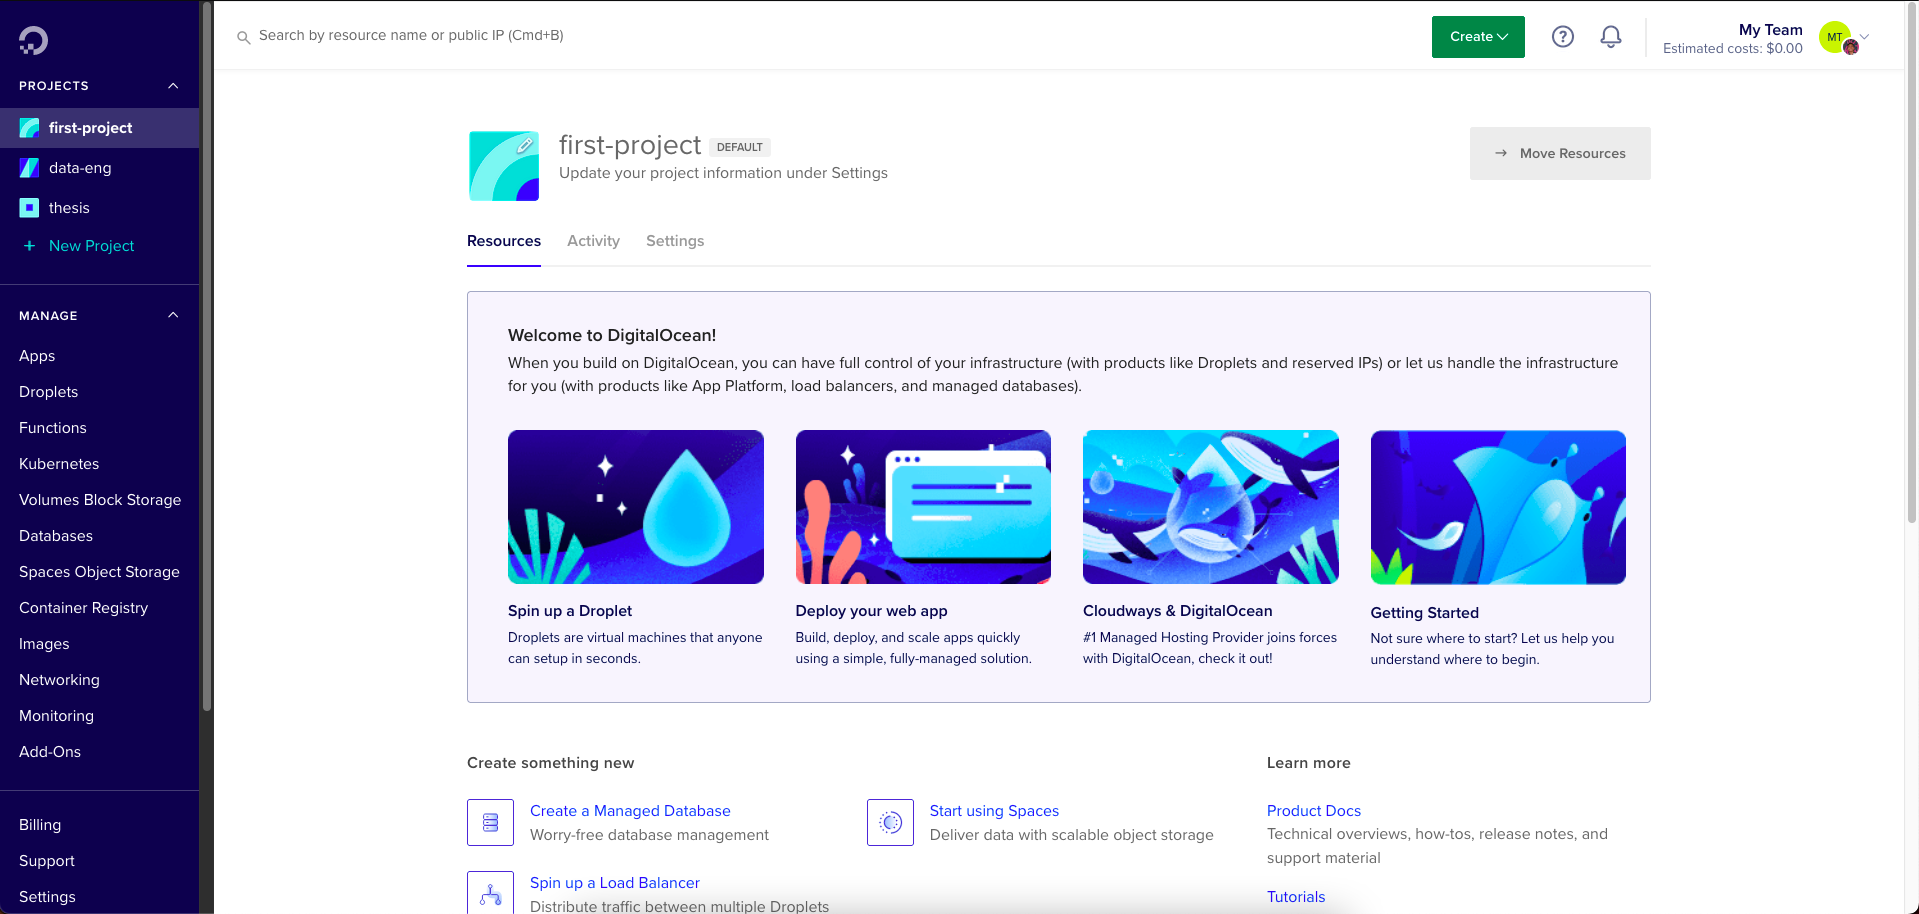
\includegraphics[width=1\linewidth]{figures/ch99/ap1/1.png}
	\end{center} 
  \item Perhatikan menu di sebelah kiri pada laman dasbor DigitalOcean. Tekan Droplets untuk masuk ke laman pembuatan VM. Selanjutnya, tekan \textit{Create Droplets} berwarna biru untuk melakukan konfigurasi VM yang akan dibuat nantinya. \pagebreak
	\begin{center}
	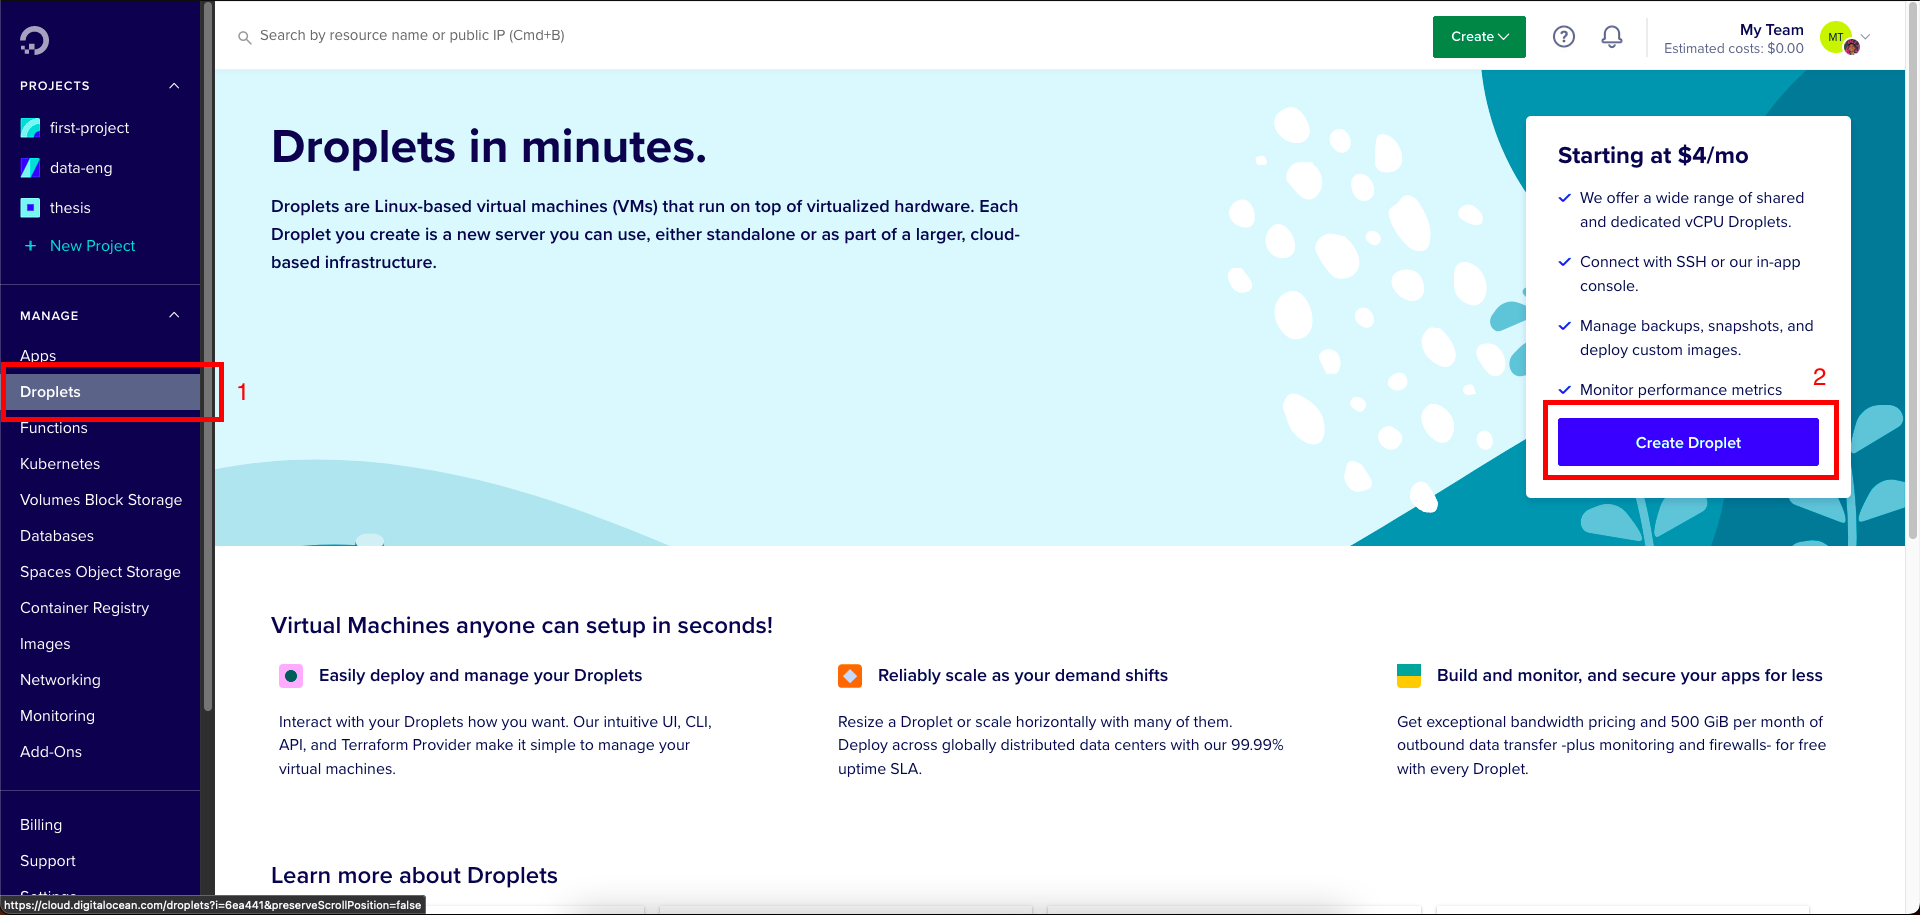
\includegraphics[width=1\linewidth]{figures/ch99/ap1/2.png}
	\end{center} 
  \item Pada laman pembuatan Droplets, lakukan konfigurasi sesuai dengan Tabel \ref{table:conf-hardware}. Jika telah selesai melakukan konfigurasi, tekan \textit{Create Droplets}. 
	\begin{center}
	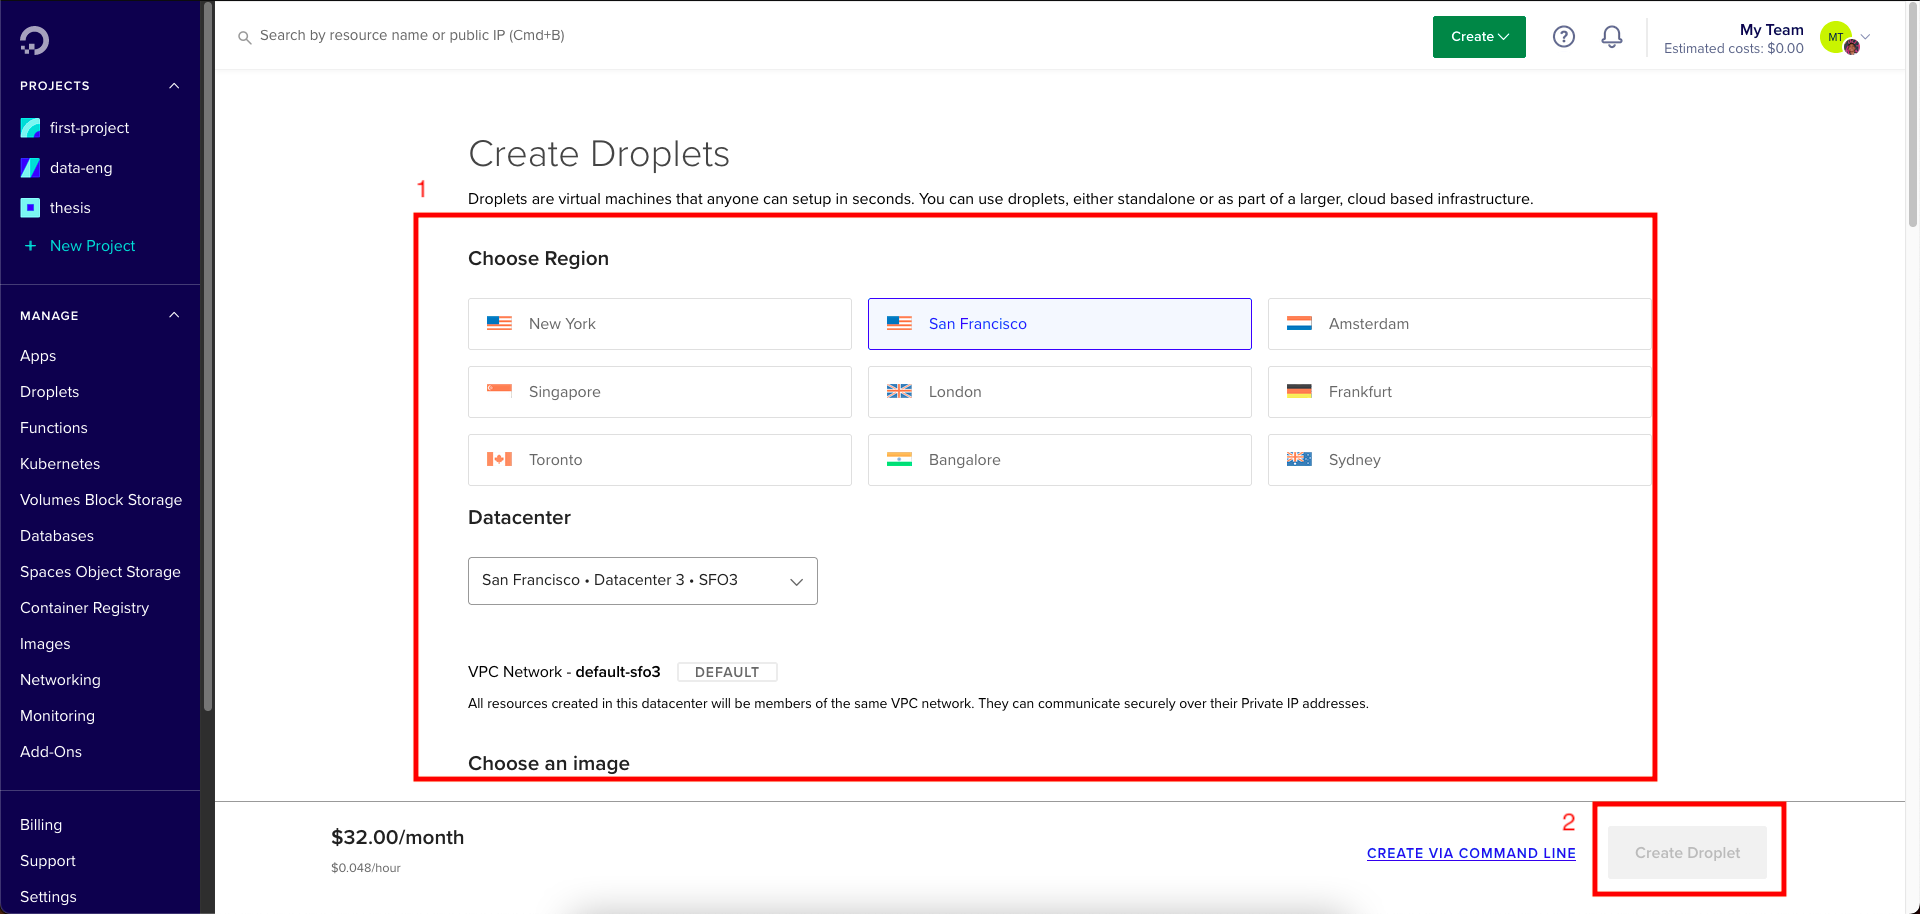
\includegraphics[width=1\linewidth]{figures/ch99/ap1/3.png}
	\end{center} 
  \item Jika pembuatan Droplets berhasil, laman dasbor \textit{Projects} DigitalOcean akan terlihat. Pada bagian Resources akan terlihat Droplets yang baru saja kita buat. Selanjutnya, tekan nama Droplets yang baru saja dibuat. 
	\begin{center}
	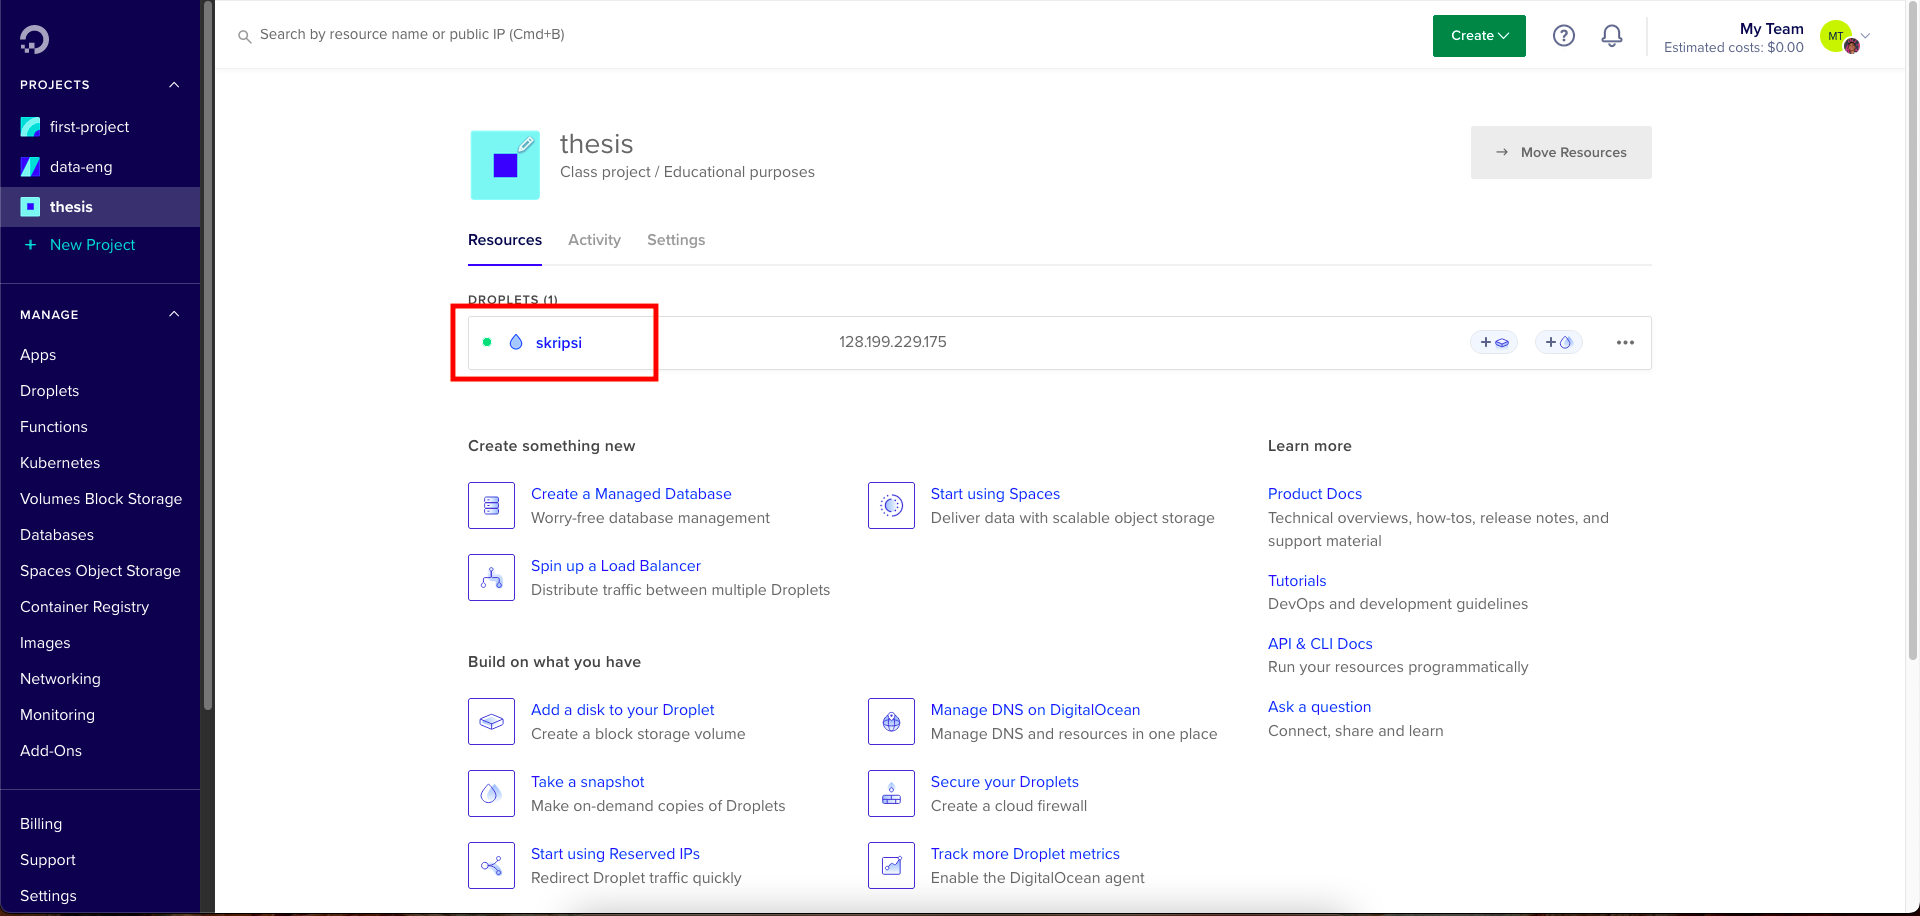
\includegraphics[width=1\linewidth]{figures/ch99/ap1/4.png}
	\end{center} 
  \item Selanjutnya, laman konfigurasi Droplets akan terlihat. Jika diperlukan konfigurasi lanjutan dapat diatur melalui laman ini. Pada tahap ini hanya akan fokus pada konfigurasi perangkat lunak tanpa konfigurasi perangkat keras lebih jauh. Untuk masuk ke VM yang sudah dibuat, tekan Console. \textit{Tab} baru akan dibuka.
	\begin{center}
	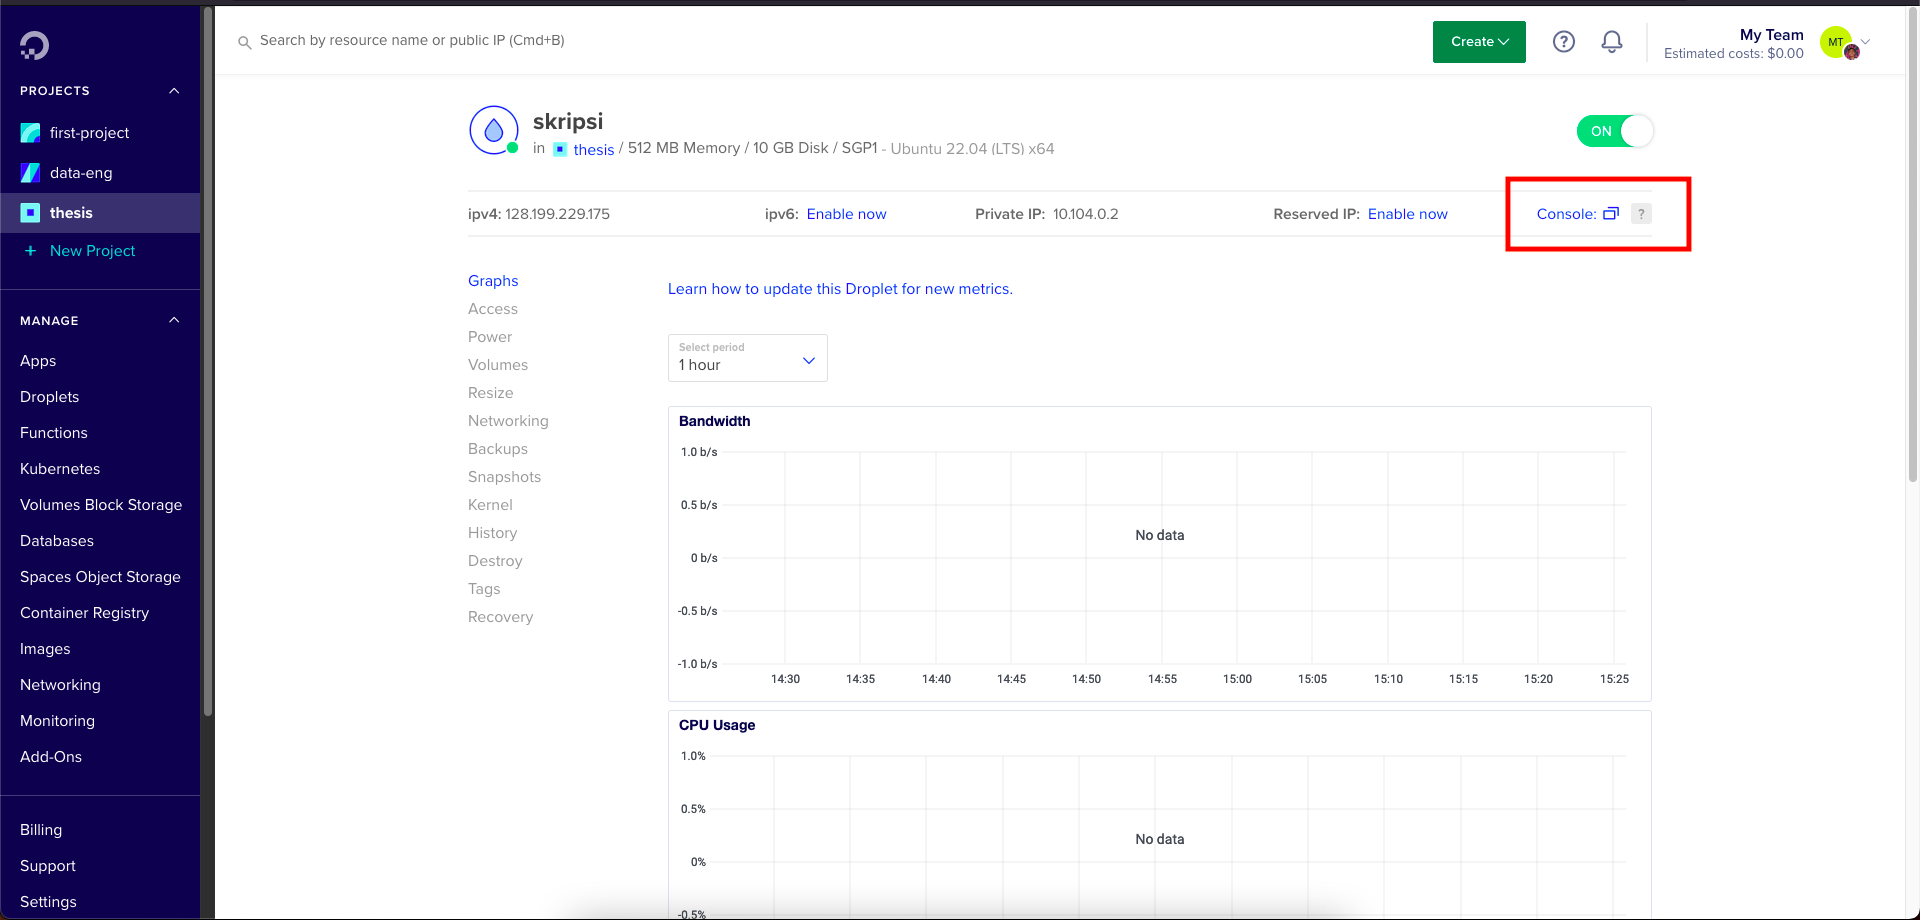
\includegraphics[width=1\linewidth]{figures/ch99/ap1/5.png}
	\end{center} 
  \item Akhirnya, lakukan konfigurasi perangkat lunak pada bagian ini.
	\begin{center}
	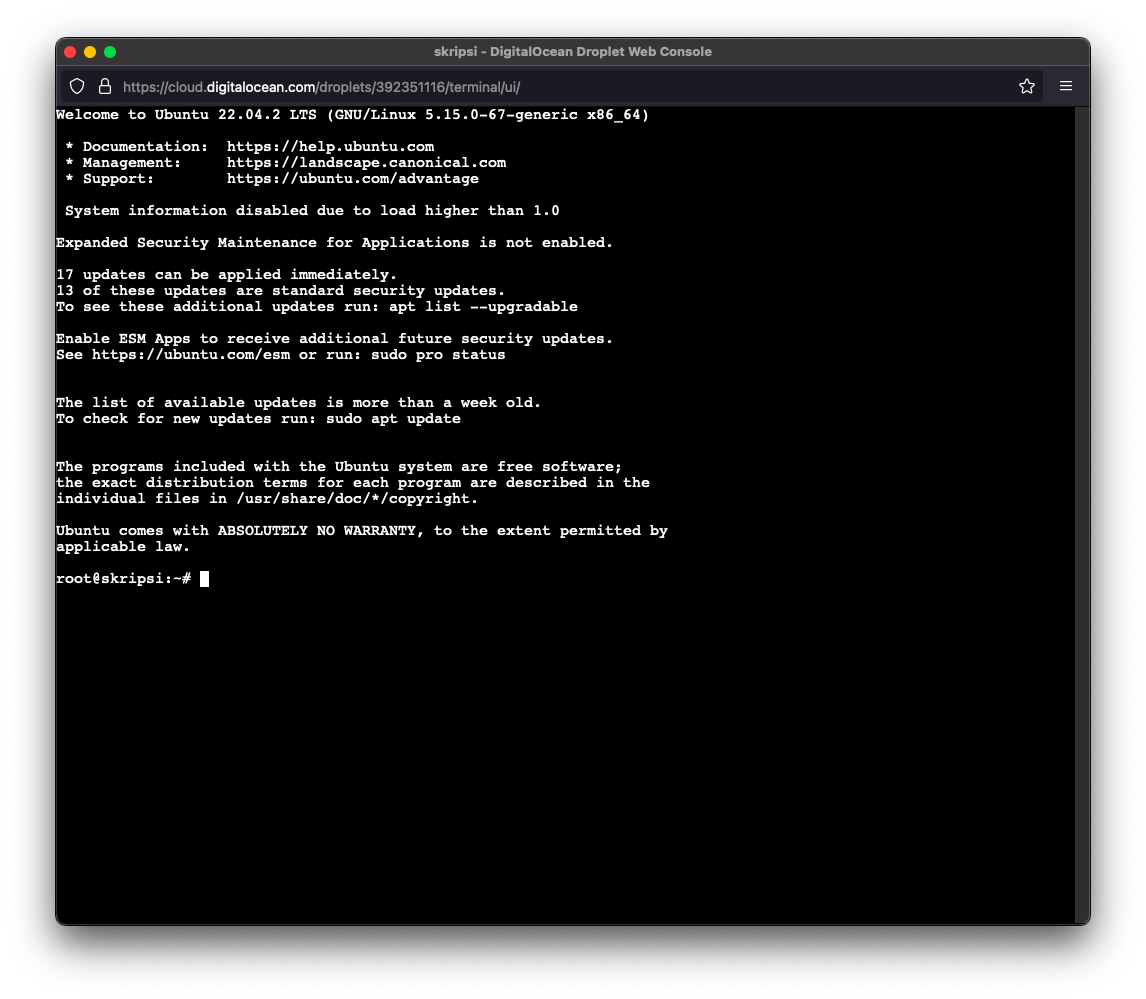
\includegraphics[width=1\linewidth]{figures/ch99/ap1/6.png}
	\end{center} 

\end{enumerate}


%-------------------------------------------------

\chapter{Instalasi dan Konfigurasi Perangkat Lunak Prasyarat}
\label{appendix:B}

Pemasangan dan konfigurasi perangkat lunak adalah hal yang krusial. Sebelum dilakukan pemasangan perangkat lunak penyimpanan dan pemrosesan \textit{big data}, tentunya perlu disiapkan perangkat lunak prasyarat. Perangkat lunak prasyarat yang dibutuhkan meliputi Git, Java dan Maven, Python, serta Scala. Langkah-langkah pemasangan dan konfigurasi perangkat lunak akan dijelaskan sebagai berikut,

\begin{enumerate}
  \item Pastikan Droplets pada DigitalOcean sudah dibuat. Masuk ke \textit{Virtual Machine} (VM) yang sebelumnya sudah dibuat melalui \textit{Console} yang berada pada laman konfigurasi Droplets DigitalOcean.
	\begin{center}
	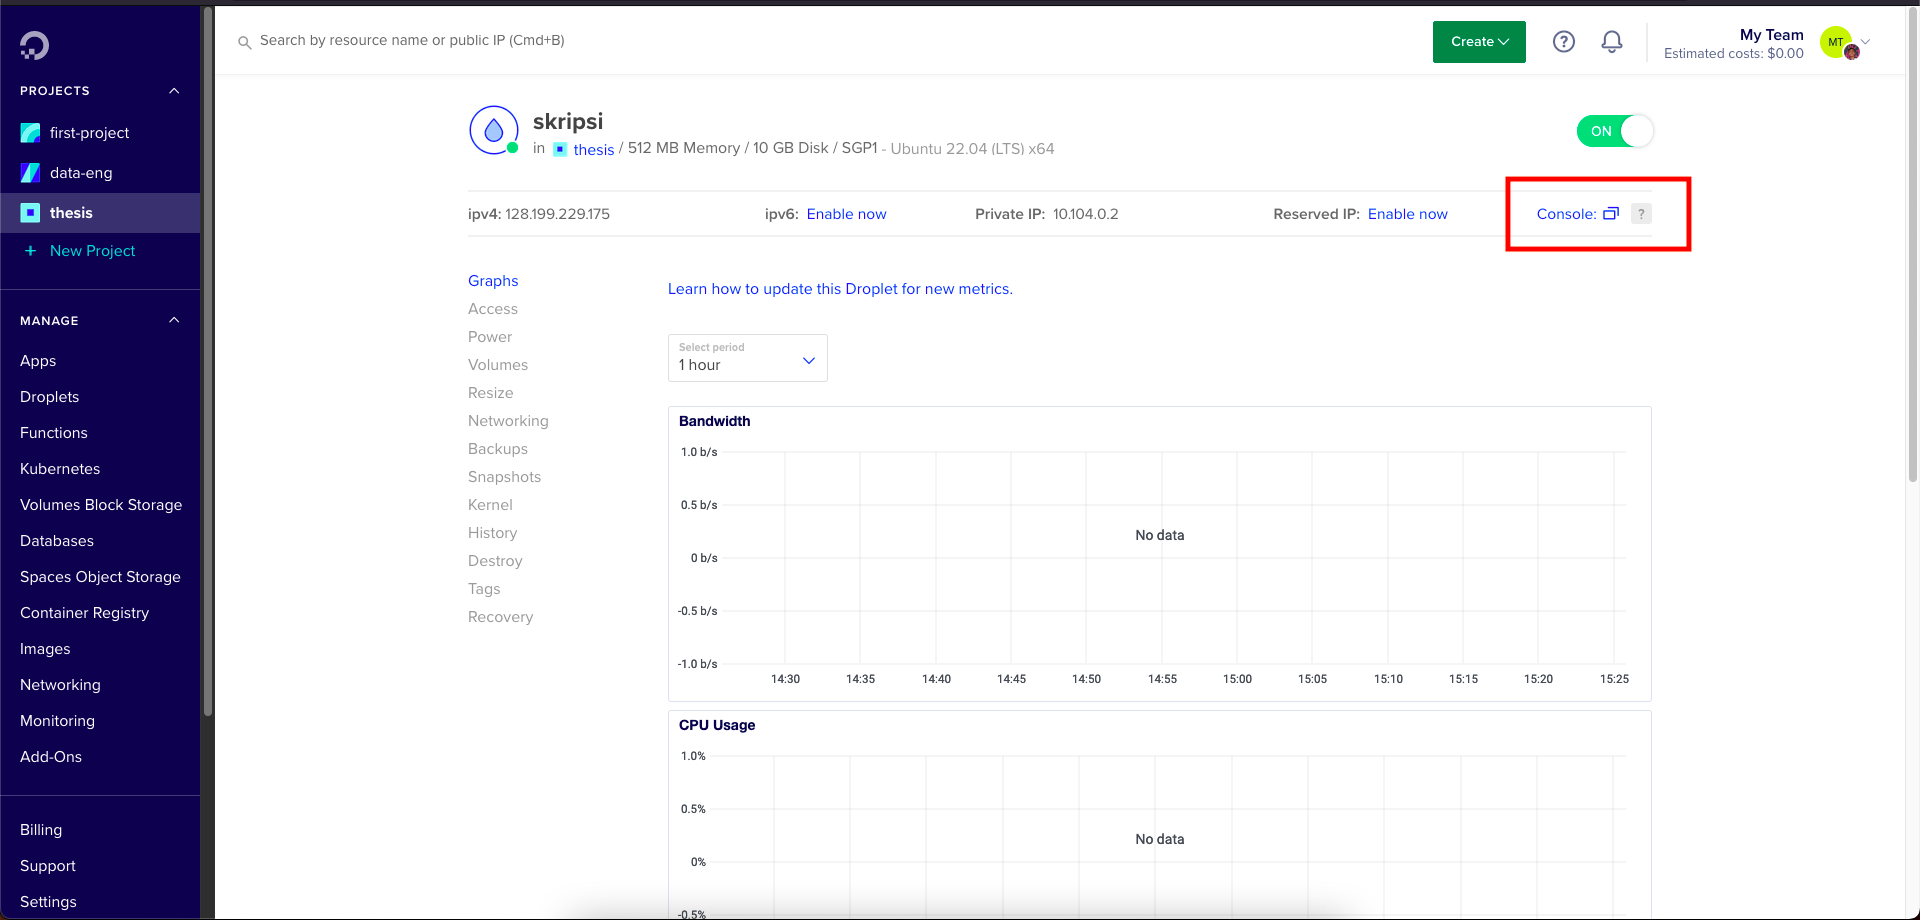
\includegraphics[width=1\linewidth]{figures/ch99/ap1/5.png}
	\end{center} 
  \item Jika Droplets baru saja dibuat, perlu dilakukan pembaruan \textit{index} pada \textit{package management}. \textit{Package management} adalah sistem atau sekumpulan alat yang digunakan untuk mengotomatiskan penginstalan, peningkatan, konfigurasi, dan penggunaan perangkat lunak. Pembaruan \textit{package management} dapat dilakukan dengan \verb|sudo apt update|. 
  \item Membuat Pengguna Baru   \begin{enumerate}
    \item Pertama, buatlah grup baru yang bernama \textit{hadoop} dengan perintah \verb|sudo addgroup hadoop|.
    \item Kemudian, tambahkan pengguna baru \textit{hdfsuser} dalam grup \textit{hadoop} yang sama dengan perintah \verb|sudo adduser --ingroup hadoop hdfsuser|.
    \item Berikan \textit{hdfsuser} izin \textit{root} yang diperlukan untuk pemasangan file. Hak istimewa pengguna \textit{root} dapat diberikan dengan memperbarui file \textit{sudoers}. Buka file \textit{sudoers} dengan menjalankan perintah \verb|sudo visudo|. Tambahkan baris berikut, yaitu \verb|hdfsuser ALL=(ALL:ALL) ALL|.
    \item Sekarang, simpan perubahan dan tutup editor.
    \item Selanjutnya, mari beralih ke pengguna baru yang telah dibuat untuk instalasi lebih lanjut menggunakan perintah \verb|su - hdfsuser|.
  \end{enumerate}
  \item Pengaturan \textit{SSH keys} untuk Hadoop
  \begin{enumerate}
  	\item Hadoop menggunakan \textit{Secure Shell} (SSH) untuk menjalankan proses antara \textit{master nodes} dan \textit{slave nodes}. Penggunaan SSH akan memberikan banyak keuntungan, salah satunya adalah kecepatan. Jika sebuah klaster aktif dan berjalan, komunikasi antar \textit{nodes} akan berjalan terlalu sering. Begitu pula dengan \textit{job tracker} yang harus sering mengirimkan informasi \textit{task to task} dengan cepat.Lakukan pemasangan ssh dan sshd dengan cara \verb|sudo apt-get install ssh| dan \verb|sudo apt-get install sshd| pada terminal.
    \item Selanjutnya, lakukan pembuatan \textit{SSH keys} dengan cara \verb|ssh-keygen -t rsa|. Jika pembuatan \textit{SSH keys} sudah dilakukan, jalankan perintah \verb|cat ~/.ssh/id_rsa.pub >> ~/.ssh/authorized_keys|.
    \item Ubah perizinan berkas dengan perintah \verb|chmod og-wx ~/.ssh/authorized_keys|.
    \item Terakhir, untuk memverifikasi koneksi aman sudah terjadi, lakukan \verb|ssh localhost|.
  \end{enumerate}
  \item Instalasi Git
  \begin{enumerate}
    \item Git dapat dipasang menggunakan perintah \verb|sudo apt install git|. Pengguna akan diminta konfirmasi untuk menginstall. Ketik \verb|y| kemudian tekan enter.
    \item Untuk mengecek versi Git, dapat menggunakan perintah \verb|git --version|.
  \end{enumerate}
  \item Instalasi Python
  \begin{enumerate}
    \item Python dapat dipasang menggunakan perintah \verb|sudo apt-get install python2 && sudo apt install python3.7|. Pengguna akan diminta konfirmasi untuk menginstall. Ketik \verb|y| kemudian tekan enter.
    \item Untuk mengecek versi Python, dapat menggunakan perintah \verb|python --version|.
  \end{enumerate}
  \item Instalasi Java 8 dan Maven
  \begin{enumerate}
    \item Java 8 dapat dipasang menggunakan perintah \verb|sudo apt install openjdk-8-jre-headless openjdk-8-jdk|. Pengguna akan diminta konfirmasi untuk menginstall. Ketik \verb|y| kemudian tekan enter.
    \item Versi dari Java dapat dilihat menggunakan perintah \verb|java -version|.
    \item Selanjutnya, instalasi Maven dapat dilakukan menggunakan perintah \verb| sudo apt-get -y install maven|.
    \item Informasi dari Maven beserta Java yang digunakan dapat dilihat menggunakan perintah \verb|mvn -version|.
  \end{enumerate}
  \item Instalasi Scala
  \begin{enumerate}
    \item Scala yang akan dipasang adalah versi 2.12. Jika menggunakan manajer paket, versi yang akan dipasang adalah versi terbaru. Untuk mengunduh versi spesifik dari Scala, dapat menggunakan perintah \verb|sudo wget  https://downloads.lightbend.com/scala/| \verb|2.12.0/scala-2.12.0.deb|.
    \item Scala dapat dipasang menggunakan perintah \verb|sudo dpkg -i scala-2.12.0.deb|.
    \item Versi Scala dapat dilihat melalui perintah \verb|scala -version|.
  \end{enumerate}
\end{enumerate}

%-------------------------------------------------

\chapter{Instalasi dan Konfigurasi Hadoop}
\label{appendix:C}

Langkah-langkah pemasangan dan konfigurasi Hadoop akan dijelaskan sebagai berikut,

\begin{enumerate}
  \item Unduh Hadoop
  \begin{enumerate}
    \item Pastikan perangkat lunak prasyarat sudah berhasil dipasang dan dilakukan konfigurasi. Sebelum dilakukan pemasangan Hadoop, diperlukan untuk mengunduh berkas Hadoop terlebih dahulu dengan perintah \verb|cd /usr/local|, dilanjutkan dengan \verb|sudo wget https://archive.apache.org/dist/hadoop/|
    \newline \verb|common/hadoop-2.4.0/hadoop-2.4.0.tar.gz|.
    \item Ekstrak berkas Hadoop yang sudah diunduh tadi dengan perintah \verb|sudo tar xvzf hadoop-2.4.0.tar.gz|. Hasil ekstrak berkas Hadoop akan disimpan pada direktori yang sama.
    \item Selanjutnya, untuk memudahkan kedepannya, ganti nama folder Hadoop dengan perintah \verb|sudo mv hadoop-2.4.0 hadoop|.
  \end{enumerate}
  \item Mengubah Kepemilikan Berkas Hadoop
  \begin{enumerate}
    \item Setelah berkas Hadoop sudah berhasil terunduh, selanjutnya ubah kepemilikan berkas Hadoop ke \textit{hdfsuser} yang sebelumnya sudah kita buat dengan perintah \verb|sudo chown -R hdfsuser:hadoop /usr/local/hadoop|.
    \item Tambahkan kekuasaaan untuk membaca, menulis, dan mengeksekusi pada foler Hadoop dengan perintah \verb|sudo chmod -R 777 /usr/local/hadoop|.
  \end{enumerate}
  \item Mematikan \textit{IPv6 Networks}
  \begin{enumerate}
    \item Saat ini Hadoop belum mendukung penggunaan \textit{IPv6 Networks}. Hadoop hanya dibangun dan diuji coba pada \textit{IPv4 Networks}. Untuk mematikan IPv6, dapat dimulai deengan menjalankan perintah \verb|cat /proc/sys/net/ipv6/conf/all/disable_ipv6|.
    \item Jika hasil yang diberikan bukan angka 1, maka beberapa langkah tambahan harus dijalankan. Jalankan perintah \verb|sudo nano /etc/sysctl.conf|, kemudian tambahkan beberapa baris potongan kode berikut pada akhir berkas,
      \begin{lstlisting}[language=bash]
    	# Disable ipv6
		net.ipv6.conf.all.disable_ipv6=1
		net.ipv6.conf.default_ipv6=1
		net.ipv6.conf.lo.disable_ipv6=1
      \end{lstlisting}
    \item Simpan berkas. Kemudian jalankan perintah \verb|sudo sysctl -p| untuk mengaktifkan perubahan.
  \end{enumerate}
  \item Menambahkan Hadoop pada \textit{Environments Variables}
  \begin{enumerate}
    \item Hadoop perlu ditambahkan pada \textit{Environments Variabels} untuk memudahkan dalam melakukan eksekusi. Untuk menambahkannya, jalankan perintah \verb|sudo nano ~/.bashrc|.
    \item Tambahkan beberapa baris kode berikut pada akhir berkas \textit{bashrc}.
      \begin{lstlisting}[language=bash]
		# HADOOP ENVIRONMENT
		export HADOOP_HOME=/usr/local/hadoop
		export HADOOP_CONF_DIR=/usr/local/hadoop/etc/hadoop
		export HADOOP_MAPRED_HOME=/usr/local/hadoop
		export HADOOP_COMMON_HOME=/usr/local/hadoop
		export HADOOP_HDFS_HOME=/usr/local/hadoop
		export YARN_HOME=/usr/local/hadoop
		export PATH=$PATH:/usr/local/hadoop/bin
		export PATH=$PATH:/usr/local/hadoop/sbin
		
		# HADOOP NATIVE PATH
		export HADOOP_COMMON_LIB_NATIVE_DIR=$HADOOP_HOME/lib/native
		export HADOOP_OPTS=-Djava.library.path=$HADOOP_PREFIX/lib
      \end{lstlisting}
    \item Untuk mendapatkan perubahan dapat dilakukan dengan perintah \verb|source ~/.bashrc|.
  \end{enumerate}
  \item Konfigurasi Hadoop
  \begin{enumerate}
    \item Hadoop mengunakan berkas .xml untuk melakukan konfigurasi pada semua prosesnya. Biasanya, letak direktori untuk melakukan konfigurasi terletak pada \verb|$HADOOP_HOME/etc/hadoop|. Oleh karena itu, jalankan perintah \verb|cd /usr/local/hadoop/etc/hadoop/|.
    \item Konfigurasi berkas \textit{hadoop-env.sh} dapat dilakukan dengan perintah \verb|sudo nano hadoop-env.sh|, dilanjutkan dengan menambahkan beberapa baris kode seperti di bawah ini,
       \begin{lstlisting}[language=bash]
		export HADOOP_OPTS=-Djava.net.preferIPv4Stack=true
		export JAVA_HOME=/usr
		export HADOOP_HOME_WARN_SUPPRESS="TRUE"
		export HADOOP_ROOT_LOGGER="WARN,DRFA"
		export HDFS_NAMENODE_USER="hdfsuser"
		export HDFS_DATANODE_USER="hdfsuser"
		export HDFS_SECONDARYNAMENODE_USER="hdfsuser"
		export YARN_RESOURCEMANAGER_USER="hdfsuser"
		export YARN_NODEMANAGER_USER="hdfsuser"
      \end{lstlisting}
    \item Konfigurasi berkas \textit{yarn-site.xml} dapat dilakukan dengan perintah \verb|sudo nano yarn-site.xml|, dilanjutkan dengan menambahkan beberapa baris kode seperti di bawah ini,
       \begin{lstlisting}[language=XML]
		<property>
		<name>yarn.nodemanager.aux-services</name>
		<value>mapreduce_shuffle</value>
		</property>
		<property>
		<name>yarn.nodemanager.aux-services.mapreduce.shuffle.class</name>
		<value>org.apache.hadoop.mapred.ShuffleHandler</value>
		</property>
      \end{lstlisting}
    \item Konfigurasi berkas \textit{hdfs-site.xml} dapat dilakukan dengan perintah \verb|sudo nano hdfs-site.xml|, dilanjutkan dengan menambahkan beberapa baris kode seperti di bawah ini,
       \begin{lstlisting}[language=XML]
		<property>
		<name>dfs.replication</name>
		<value>1</value>
		</property>
		<property>
		<name>dfs.namenode.name.dir</name>
		<value>/usr/local/hadoop/yarn_data/hdfs/namenode</value>
		</property>
		<property>
		<name>dfs.datanode.data.dir</name>
		<value>/usr/local/hadoop/yarn_data/hdfs/datanode</value>
		</property>
		<property>
		<name>dfs.namenode.http-address</name>
		<value>localhost:50070</value>
		</property>
      \end{lstlisting}
    \item Konfigurasi berkas \textit{core-site.xml} dapat dilakukan dengan perintah \verb|sudo nano core-site.xml|, dilanjutkan dengan menambahkan beberapa baris kode seperti di bawah ini,
       \begin{lstlisting}[language=XML]
		<property>
		<name>hadoop.tmp.dir</name>
		<value>/bigdata/hadoop/tmp</value>
		</property>
		<property>
		<name>fs.default.name</name>
		<value>hdfs://localhost:9000</value>
		</property>
      \end{lstlisting}
    \item Konfigurasi berkas \textit{mapred-site.xml} dapat dilakukan dengan perintah \verb|sudo nano mapred-site.xml|, dilanjutkan dengan menambahkan beberapa baris kode seperti di bawah ini,
       \begin{lstlisting}[language=XML]
		<property>
		<name>mapred.framework.name</name>
		<value>yarn</value>
		</property>
		<property>
		<name>mapreduce.jobhistory.address</name>
		<value>localhost:10020</value>
		</property>
      \end{lstlisting}
  \end{enumerate}
  \item Membuat Direktori Hadoop untuk Menyimpan Data
  \begin{enumerate}
    \item Sesuai dengan apa yang ditulis pada \textit{core-site.xml}, langkah pertama yang harus dilakukan adalah membuat direktori sementara untuk dfs menyimpan berkas dengan menjalankan perintah di bawah. Jalankan perintah berikut baris per baris.
       \begin{lstlisting}[language=bash]
		sudo mkdir -p /bigdata/hadoop/tmp
		sudo chown -R hdfsuser:hadoop /bigdata/hadoop/tmp
		sudo chmod -R 777 /bigdata/hadoop/tmp
      \end{lstlisting}
    \item Selanjutnya, jalankan perintah berikut untuk membuat direktori untuk menyimpan berkas data sekaligus mengganti kepemilikan berkas. Jalankan perintah berikut baris per baris.
       \begin{lstlisting}[language=bash]
		sudo mkdir -p /usr/local/hadoop/yarn_data/hdfs/namenode
		sudo mkdir -p /usr/local/hadoop/yarn_data/hdfs/datanode
		sudo chmod -R 777 /usr/local/hadoop/yarn_data/hdfs/namenode
		sudo chmod -R 777 /usr/local/hadoop/yarn_data/hdfs/datanode
		sudo chown -R hdfsuser:hadoop /usr/local/hadoop/yarn_data/hdfs/namenode
		sudo chown -R hdfsuser:hadoop /usr/local/hadoop/yarn_data/hdfs/datanode
      \end{lstlisting}
    \item Konfigurasi untuk Hadoop sudah selesai dan dapat dilanjutkan untuk menjalankan \textit{Resource Manager} dan \textit{Node Manager}
  \end{enumerate}
  \item Menjalankan Hadoop
  \begin{enumerate}
    \item Sebelum menjalankan \textit{Hadoop Core Services}, klaster harus dibersihkan dengan cara melakukan \textit{format} pada \textit{namenode}. Jalankan perintah \verb|hdfs namenode -format|.
    \item Untuk menjalankan layanan Hadoop, dapat dilakukan dengan perintah \verb|start-all.sh|.
    \item Perintah \verb|jps| dapat dilakukan untuk mengecek apakah layanan Hadoop sudah berjalan.
    \item Untuk memberhentikan layanan Hadoop, dapat dilakukan dengan perintah \verb|stop-all.sh| pada terminal.
  \end{enumerate}
\end{enumerate}

%-------------------------------------------------


\chapter{Instalasi dan Konfigurasi Spark}
\label{appendix:D}

Langkah-langkah pemasangan dan konfigurasi Spark akan dijelaskan sebagai berikut,

\begin{enumerate}
  \item Unduh Berkas Spark
  \begin{enumerate}
    \item Pastikan perangkat lunak prasyarat sudah berhasil dipasang dan dilakukan konfigurasi. Sebelum dilakukan pemasangan Spark, diperlukan untuk mengunduh berkas Spark terlebih dahulu dengan perintah \verb|cd /usr/local|, dilanjutkan dengan \verb|sudo wget https://archive.apache.org/dist/spark/|
    \newline \verb|spark-2.1.3/spark-2.1.3-bin-hadoop2.4.tgz|.    
    \item Ekstrak berkas Spark yang sudah diunduh tadi dengan perintah \verb|sudo tar xvf spark-2.1.3-bin-hadoop2.4.tgz|. Hasil ekstrak berkas Spark akan disimpan pada direktori yang sama.
    \item Selanjutnya, untuk memudahkan kedepannya, ganti nama folder Spark dengan perintah \verb|sudo mv spark-2.1.3-bin-hadoop2.4  spark|. 
  \end{enumerate}
  \item Menambahkan Spark pada \textit{Environments Variables}
  \begin{enumerate}
    \item Spark perlu ditambahkan pada \textit{Environments Variabels} untuk memudahkan dalam melakukan eksekusi. Untuk menambahkannya, jalankan perintah \verb|sudo nano ~/.bashrc|.
    \item Tambahkan beberapa baris kode berikut pada akhir berkas \textit{bashrc}.
      \begin{lstlisting}[language=bash]
		# SPARK ENVIRONMENT
		export PATH=$PATH:/usr/local/spark/bin
		export YARN_CONF_DIR=$HADOOP_HOME/etc/hadoop
		export SPARK_HOME=$PATH:/usr/local/spark/bin
      \end{lstlisting}
    \item Untuk mendapatkan perubahan dapat dilakukan dengan perintah \verb|source ~/.bashrc|.
  \end{enumerate}
  \item Menjalankan \textit{Spark Shell}
  \begin{enumerate}
    \item Pastikan bahwa Spark sudah ditambahkan pada \textit{environmens variables} dengan perintah \verb|spark-submit --version|.
    \item Jalankan layanan Hadoop dengan perintah \verb|start-all.sh|.
    \item Jalankan \textit{spark-shell} dengan YARN menggunakan perintah \verb|spark-shell --master yarn|.
  \end{enumerate}
\end{enumerate}


%-------------------------------------------------


\chapter{Instalasi dan Konfigurasi HiBench}
\label{appendix:E}

Langkah-langkah pemasangan dan konfigurasi HiBench akan dijelaskan sebagai berikut,

\begin{enumerate}
  \item Unduh berkas HiBench
  \begin{enumerate}
    \item Pastikan perangkat lunak prasyarat dan perangkat lunak \textit{Big Data} sebelumnya sudah berhasil dipasang dan dilakukan konfigurasi. Tahap selanjutnya adalah mengunduh berkas HiBench dengan perintah \verb|git clone https://github.com/Intel-bigdata/HiBench.git|. Pastikan berada pada folder \textit{/home/hdfsuser}.
    \item Selanjutnya, berikan perizinan ke folder HiBench dengan cara \verb|sudo chmod 755 HiBench|.
  \end{enumerate}
  \item Membangun \textit{framework benchmark}
  \begin{enumerate}
    \item Sebelum HiBench dapat digunakan, diperlukan pembangunan beberapa modul yang dibutuhkan, misalnya modul \textit{data generation}, modul \textit{hadoopbench}, dan modul \textit{sparkbench}. Langkah awal yang diperlukan adalah masuk ke folder HiBench dengan perintah \verb|cd HiBench|.
    \item Selanjutnya, pastikan versi Hadoop, Spark, dan Scala sudah sesuai. Jalankan perintah \verb|mvn -Phadoopbench -Psparkbench -Dhadoop=2.4 -Dspark=2.1| \newline \verb|-Dmodules -Pmicro clean package|. Perintah ini akan membangun modul yang dibutuhkan menggunakan Maven. Tidak semua modul akan dipasang. Modul yang akan dipasang salah satunya adalah modul untuk \textit{micro benchmark}. 
    \item Jika ingin pembangunan modul yang lebih luas cakupannya dapat menggunakan perintah \verb|mvn -Phadoopbench -Psparkbench -Dspark=2.1 -Dscala=2.11| \newline \verb|clean package|.
  \end{enumerate}
  \item Jalankan perintah \verb |sudo apt install bc| supaya berkas Hibench \textit{Report} dapat muncul. 
  \item Lakukan konfigurasi pada berkas \textit{hibench.conf}. Buka berkas tersebut dengan perintah \verb|sudo nano conf/hibench.conf|.
  \item Lakukan beberapa perubahan pada baris sesuai dengan contoh di bawah ini.
    \begin{lstlisting}[language=bash]
	  hibench.masters.hostnames       hdfs://localhost:9000
	  hibench.slaves.hostnames        localhost
    \end{lstlisting}
  \item Menjalankan \textit{Benchmark} Hadoop
  \begin{enumerate}
    \item Lakukan konfigurasi pada berkas \textit{hadoop.conf}. Sebelum itu, salin \textit{template} konfigurasinya dengan perintah \verb|cp conf/hadoop.conf.template conf/hadoop.conf|.
    \item Buka berkas \textit{hadoop.conf} dengan perintah \verb|sudo nano conf/hadoop.conf|. Selanjutnya, lakukan beberapa perubahan seperti pada contoh di bawah.
      \begin{lstlisting}[language=bash]
		# Hadoop home
		hibench.hadoop.home     /usr/local/hadoop
		
		# The path of hadoop executable
		hibench.hadoop.executable     ${hibench.hadoop.home}/bin/hadoop
		
		# Hadoop configraution directory
		hibench.hadoop.configure.dir  ${hibench.hadoop.home}/etc/hadoop
		
		# The root HDFS path to store HiBench data
		hibench.hdfs.master       hdfs://localhost:9000
		
		# Hadoop release provider. Supported value: apache
		hibench.hadoop.release    apache
      \end{lstlisting}
    \item Simpan perubahan yang sudah dilakukan.
    \item Untuk menjalankan beban kerja yang sudah dirancang sebelumnya, perintah yang digunakan sebagai berikut. Jalankan baris per baris.
      \begin{lstlisting}[language=bash]
	    bin/workloads/micro/<nama-beban-kerja>/prepare/prepare.sh
	    bin/workloads/micro/<nama-beban-kerja>/hadoop/run.sh
      \end{lstlisting}
    \item Untuk melihat hasil dari \textit{benchmark} dapat mengakses berkas pada \verb|<HiBench_Root>/report/hibench.report|
  \end{enumerate}
  \item Menjalankan \textit{Benchmark} Spark
  \begin{enumerate}
    \item Lakukan konfigurasi pada berkas \textit{spark.conf}. Sebelum itu, salin \textit{template} konfigurasinya dengan perintah \verb|cp conf/spark.conf.template conf/spark.conf|.
    \item Buka berkas \textit{spark.conf} dengan perintah \verb|sudo nano conf/spark.conf|. Selanjutnya, lakukan beberapa perubahan seperti pada contoh di bawah.
      \begin{lstlisting}[language=bash]
		# Spark home
		hibench.spark.home      /usr/local/spark
		
		# Spark master
		#   standalone mode: spark://xxx:7077
		#   YARN mode: yarn-client
		hibench.spark.master    yarn-client
      \end{lstlisting}
    \item Simpan perubahan yang sudah dilakukan.
    \item Untuk menjalankan beban kerja yang sudah dirancang sebelumnya, perintah yang digunakan sebagai berikut. Jalankan baris per baris.
      \begin{lstlisting}[language=bash]
	    bin/workloads/micro/<nama-beban-kerja>/prepare/prepare.sh
	    bin/workloads/micro/<nama-beban-kerja>/spark/run.sh
      \end{lstlisting}
    \item Untuk melihat hasil dari \textit{benchmark} dapat mengakses berkas pada \verb|<HiBench_Root>/report/hibench.report|
  \end{enumerate}
\end{enumerate}




%-------------------------------------------------


\chapter{Skrip Otomatisasi Eksperimen}
\label{appendix:F}

\begin{lstlisting}[language=bash]
#!/bin/bash

# Ubah direktori kerja ke direktori HiBench
cd /home/hadoop/HiBench-HiBench-7.0

# Daftar workload
workloads=("wordcount" "sort")

# Daftar skala
scales=(
    "seratuskb"
    "limaratuskb"
    "satumb"
    "limamb"
    "sepuluhmb"
    "limapuluhmb"
    "seratusmb"
    "halfgig"
    "onegig"
    "fivegig"
    "tengig"
    "fiveteengig"
)

# Jumlah pengulangan
repetitions=5

# Looping untuk setiap workload
for workload in "${workloads[@]}"; do
    echo "Menjalankan workload: $workload"

    # Looping untuk setiap skala
    for scale in "${scales[@]}"; do
        echo "  Skala: $scale"

        # Mengubah konfigurasi HiBench
        sed -i "s/^hibench.scale.profile.*/hibench.scale.profile $scale/" conf/hibench.conf

        # Tahap persiapan Hadoop
        while true; do
            bin/workloads/micro/$workload/prepare/prepare.sh
            if [[ $? -eq 0 ]]; then
                break
            fi
            echo "    Tahap persiapan Hadoop gagal. Mencoba lagi..."
        done

        # Looping untuk setiap pengulangan Hadoop
        for ((i = 1; i <= repetitions; i++)); do
            echo "    Percobaan Hadoop $i"

            # Mulai dool di latar belakang
            nohup /home/hadoop/bin/dool --all --io --output "$workload-$scale-$i-hadoop.csv" --bytes > /dev/null 2>&1 &
            dool_pid=$!  # Menyimpan PID proses dool

            # Menjalankan benchmark Hadoop
            bin/workloads/micro/$workload/hadoop/run.sh

            # Menghentikan dool setelah benchmark selesai
            kill $dool_pid
            wait $dool_pid 2>/dev/null
        done

        # Tahap persiapan Spark 
        while true; do
            bin/workloads/micro/$workload/prepare/prepare.sh
            if [[ $? -eq 0 ]]; then
                break
            fi
            echo "    Tahap persiapan Spark gagal. Mencoba lagi..."
        done

        # Looping untuk setiap pengulangan Spark
        for ((i = 1; i <= repetitions; i++)); do
            echo "    Percobaan Spark $i"

            # Mulai dool di latar belakang
            nohup /home/hadoop/bin/dool --all --io --output "$workload-$scale-$i-spark.csv" --bytes > /dev/null 2>&1 &
            dool_pid=$!

            # Menjalankan benchmark Spark
            bin/workloads/micro/$workload/spark/run.sh

            # Menghentikan dool setelah benchmark selesai
            kill $dool_pid
            wait $dool_pid 2>/dev/null
        done

	# Tunggu 15 detik sebelum beralih ke skala berikutnya
	sleep 15
    done
done

echo "Selesai."
\end{lstlisting}



%-------------------------------------------------


\chapter{Visualisasi Utilisasi Sistem Sesuai Input Data (\textit{Sort})}
\label{appendix:G}

\begin{figure}[h]
    \centering
    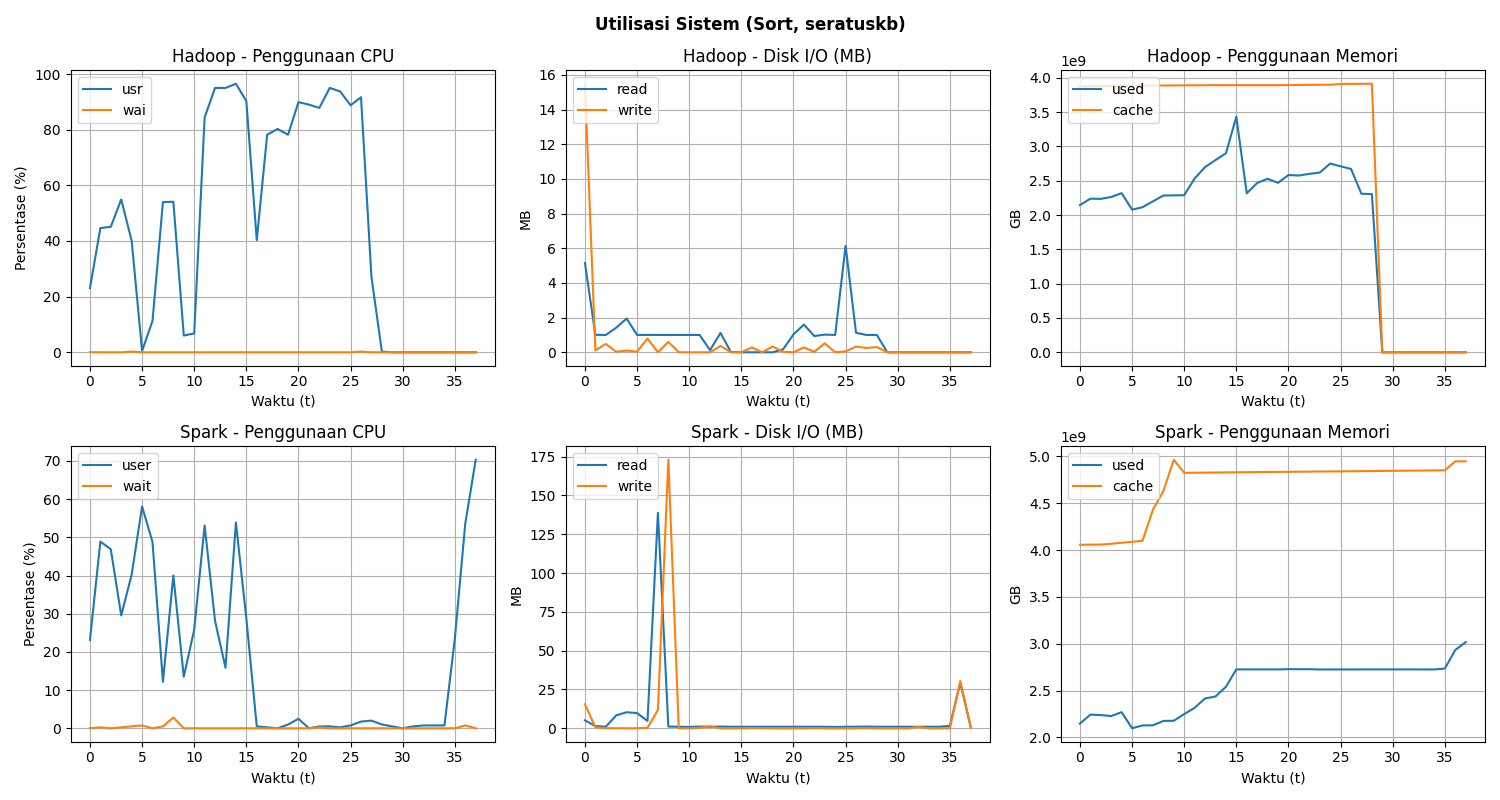
\includegraphics[width=0.9\textwidth]{figures/ch04/5-util-sistem-sort-seratuskb.png}
    \caption*{Sort, 100 KB}
\end{figure}

\begin{figure}[h]
    \centering
    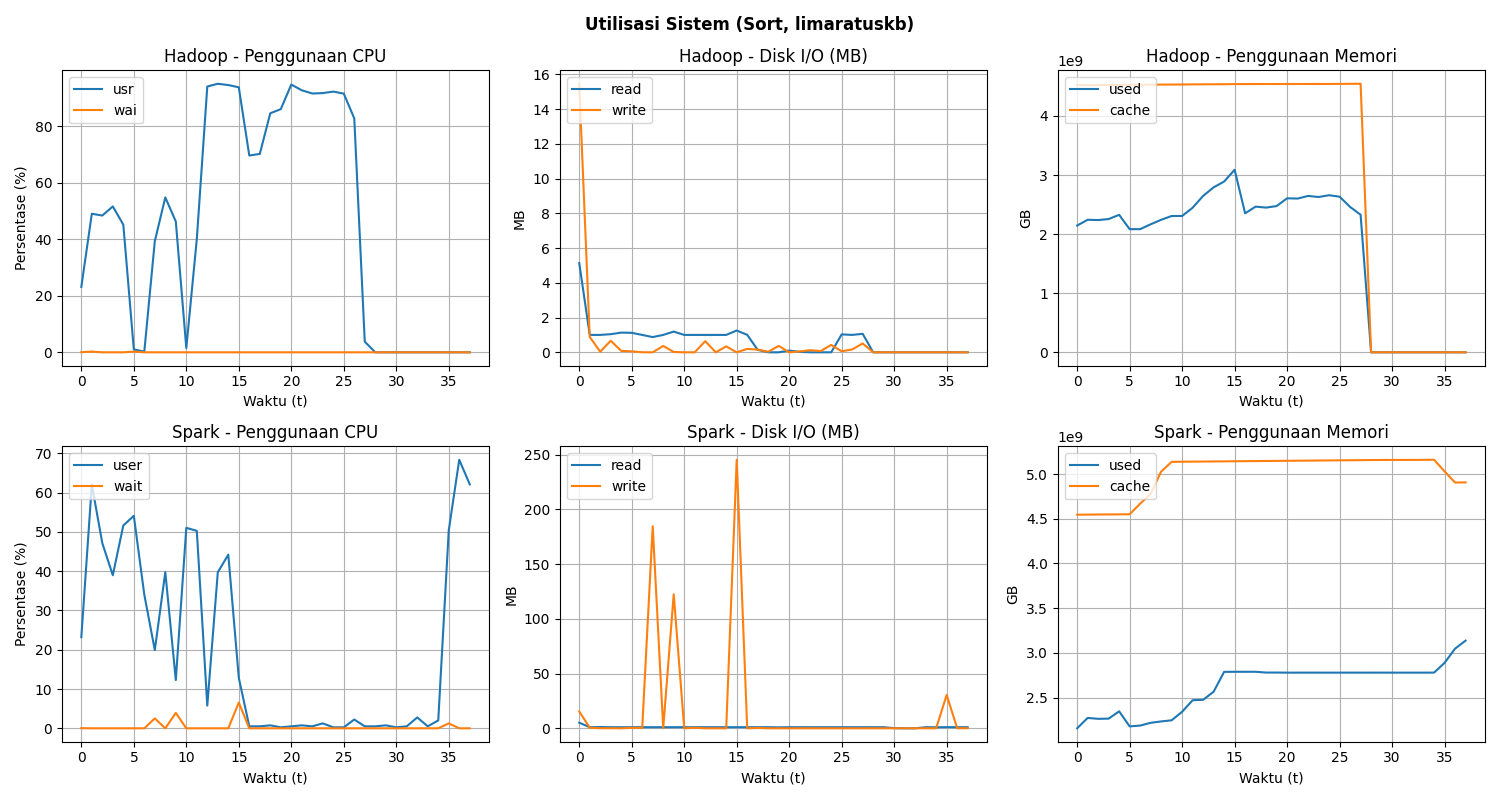
\includegraphics[width=0.9\textwidth]{figures/ch04/5-util-sistem-sort-limaratuskb.png}
    \caption*{Sort, 500 KB}
\end{figure}

\begin{figure}[h]
    \centering
    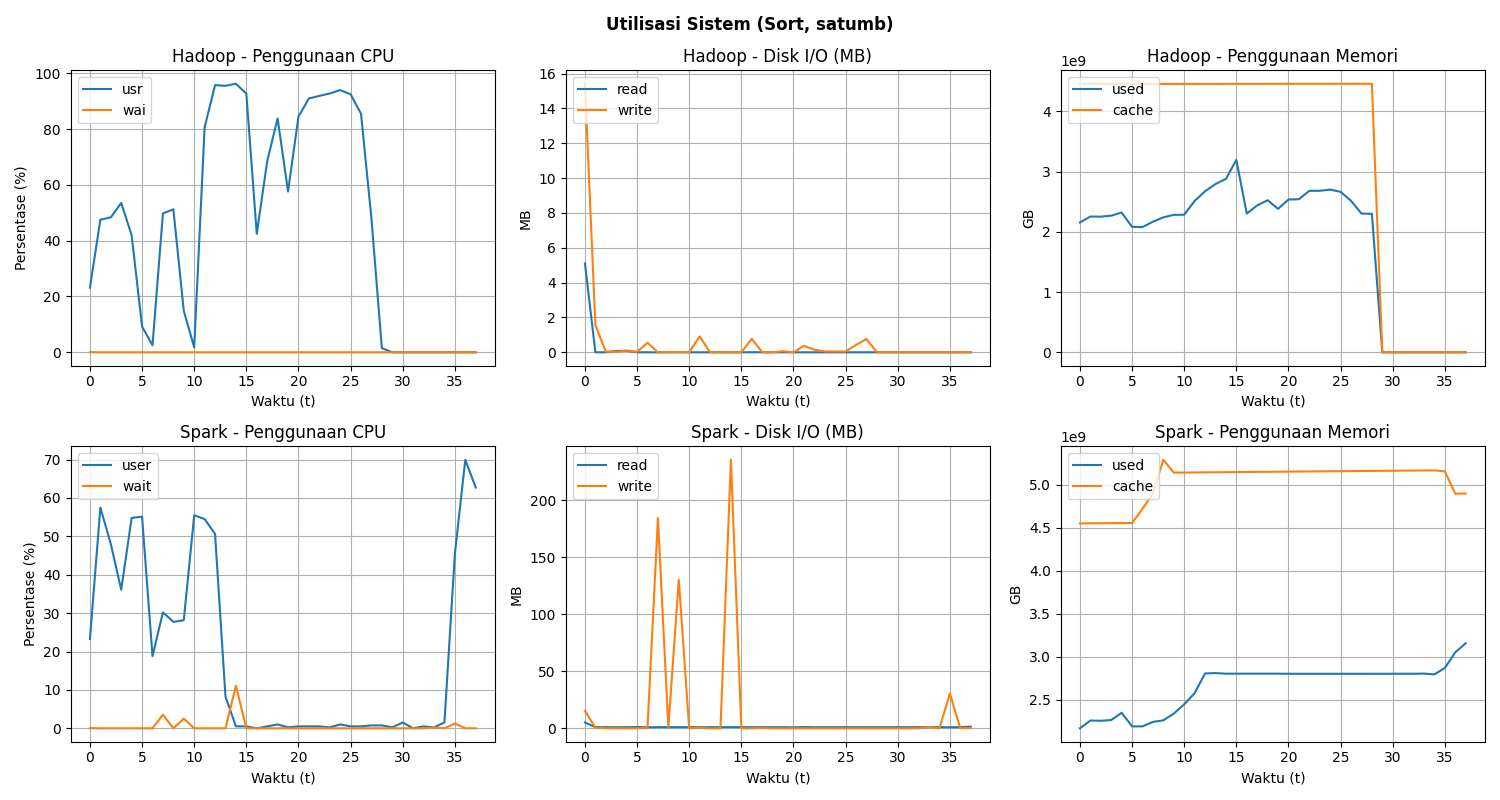
\includegraphics[width=0.9\textwidth]{figures/ch04/5-util-sistem-sort-satumb.png}
    \caption*{Sort, 1 MB}
\end{figure}

\begin{figure}[h]
    \centering
    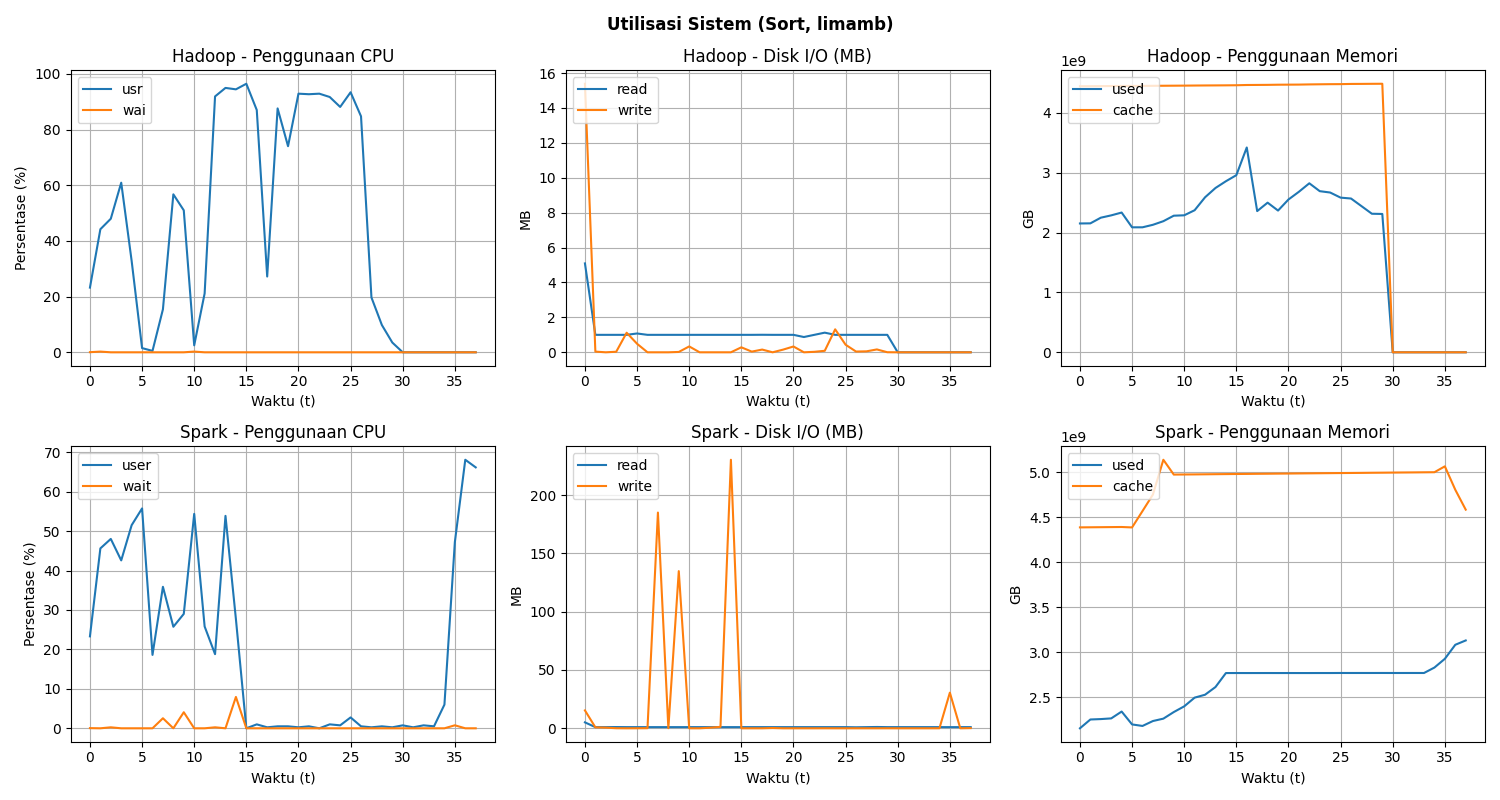
\includegraphics[width=0.9\textwidth]{figures/ch04/5-util-sistem-sort-limamb.png}
    \caption*{Sort, 5 MB}
\end{figure}

\begin{figure}[h]
    \centering
    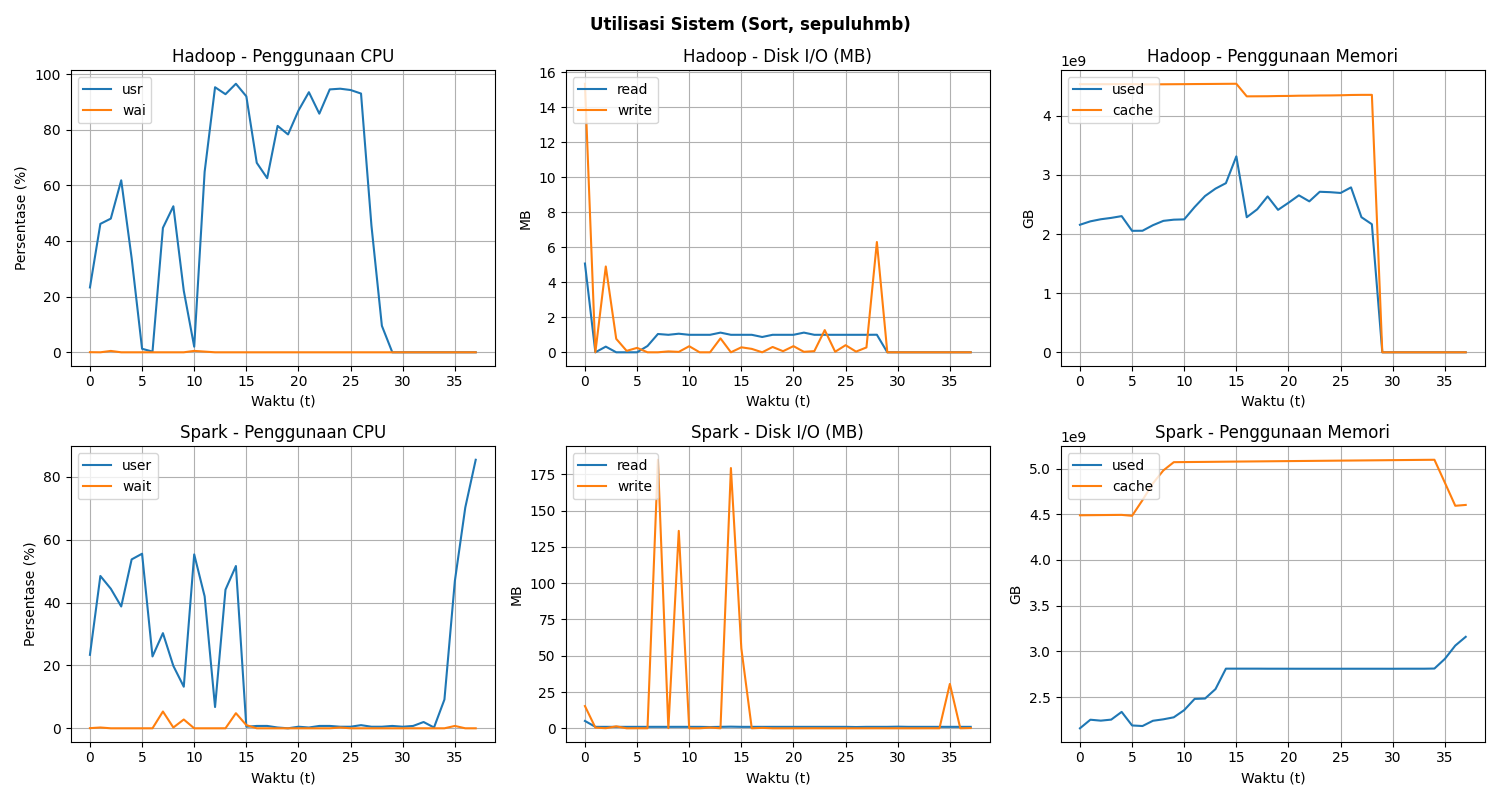
\includegraphics[width=0.9\textwidth]{figures/ch04/5-util-sistem-sort-sepuluhmb.png}
    \caption*{Sort, 10 MB}
\end{figure}

\begin{figure}[h]
    \centering
    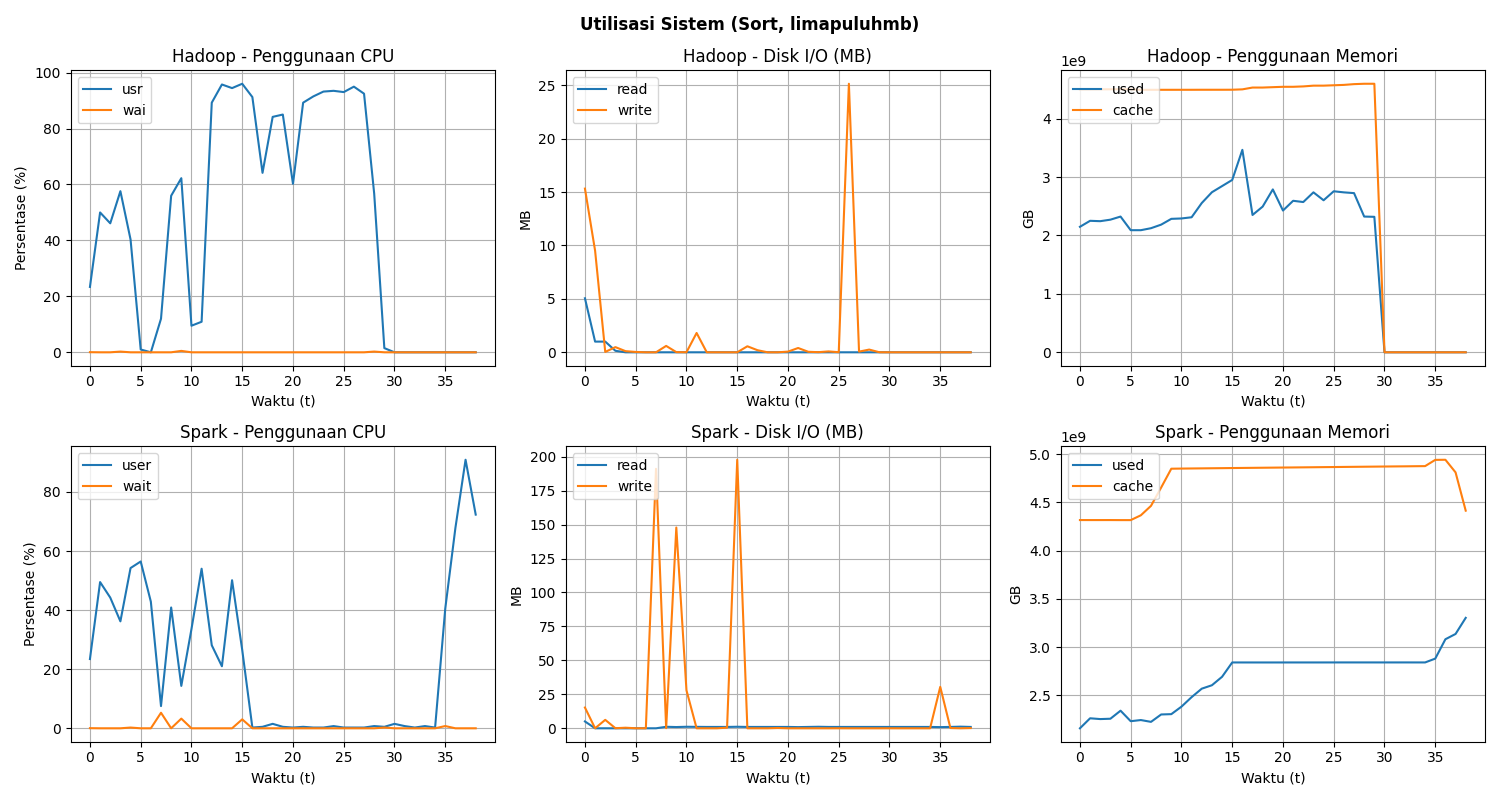
\includegraphics[width=0.9\textwidth]{figures/ch04/5-util-sistem-sort-limapuluhmb.png}
    \caption*{Sort, 50 MB}
\end{figure}

\begin{figure}[h]
    \centering
    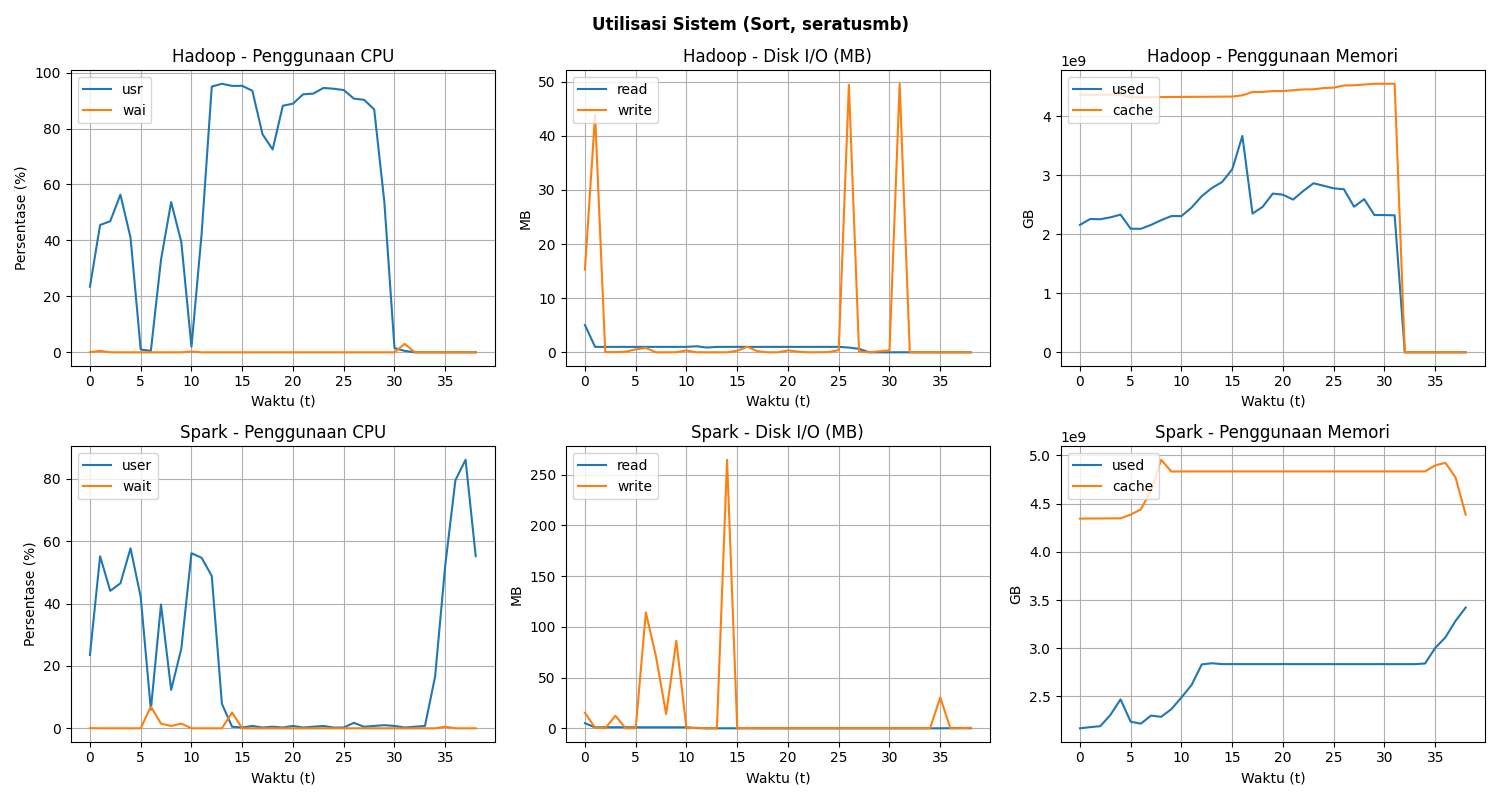
\includegraphics[width=0.9\textwidth]{figures/ch04/5-util-sistem-sort-seratusmb.png}
    \caption*{Sort, 100 MB}
\end{figure}

\begin{figure}[h]
    \centering
    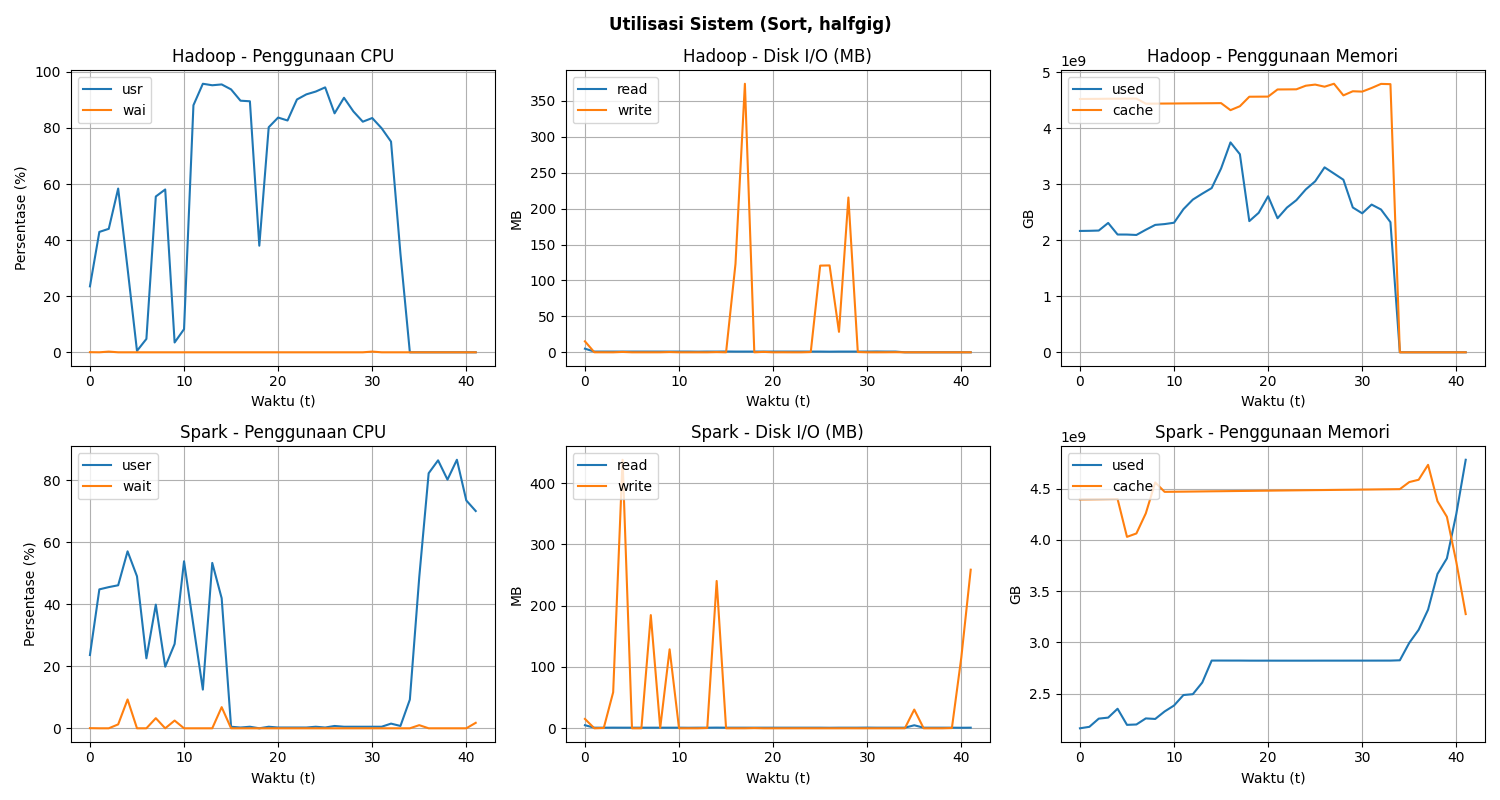
\includegraphics[width=0.9\textwidth]{figures/ch04/5-util-sistem-sort-halfgig.png}
    \caption*{Sort, 500 MB}
\end{figure}

\begin{figure}[h]
    \centering
    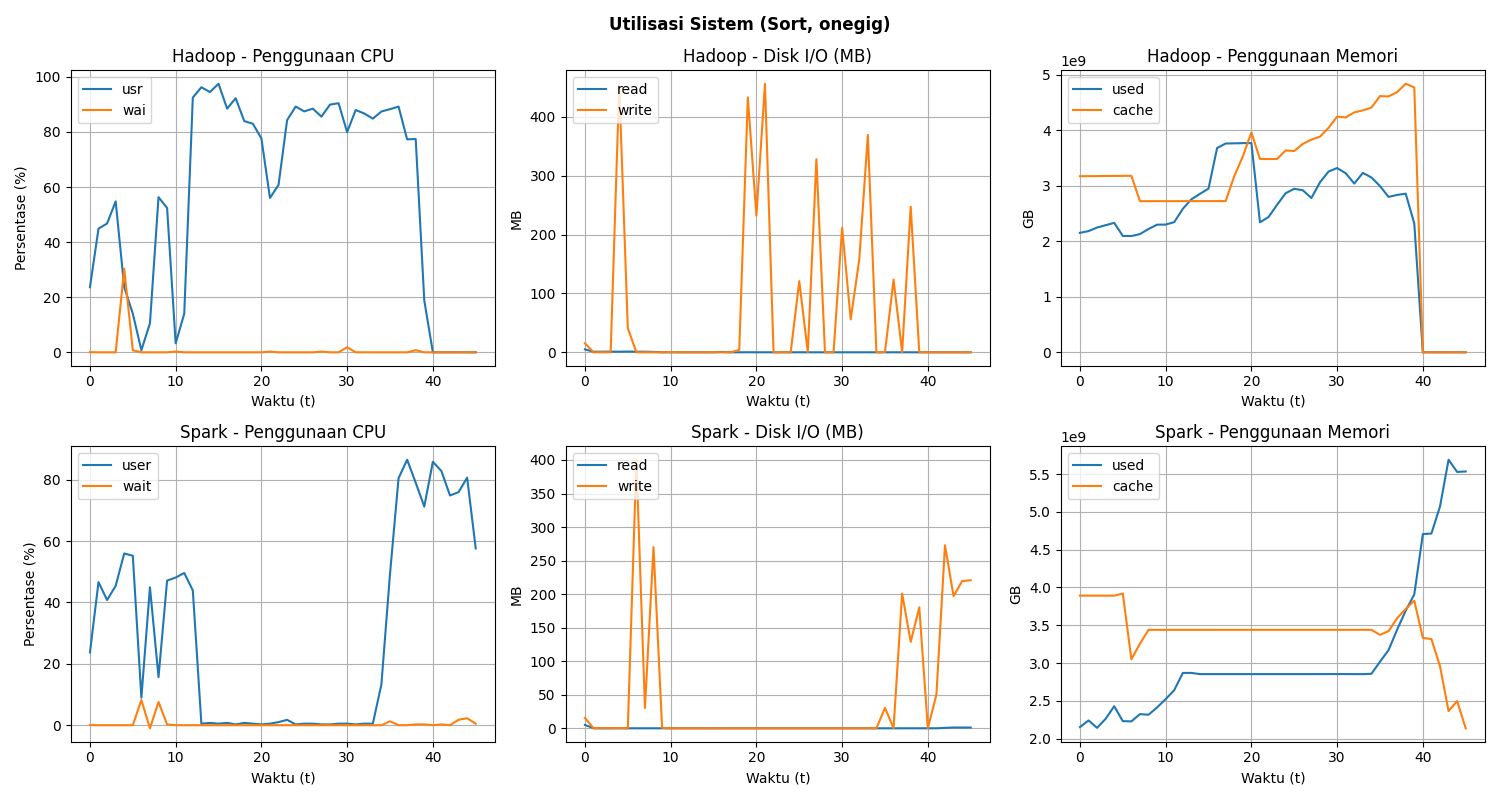
\includegraphics[width=0.9\textwidth]{figures/ch04/5-util-sistem-sort-onegig.png}
    \caption*{Sort, 1 GB}
\end{figure}

\begin{figure}[h]
    \centering
    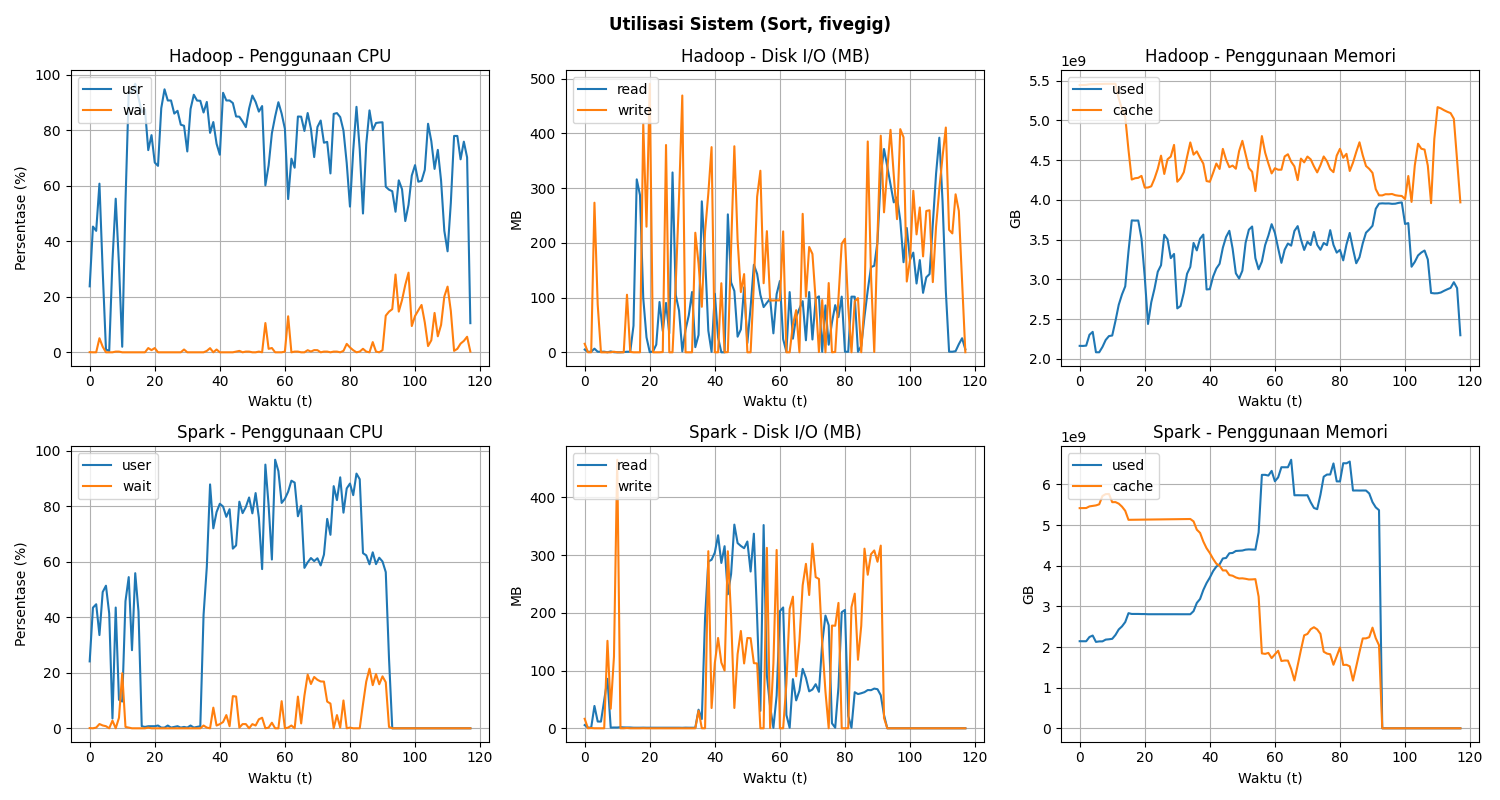
\includegraphics[width=0.9\textwidth]{figures/ch04/5-util-sistem-sort-fivegig.png}
    \caption*{Sort, 5 GB}
\end{figure}

\begin{figure}[h]
    \centering
    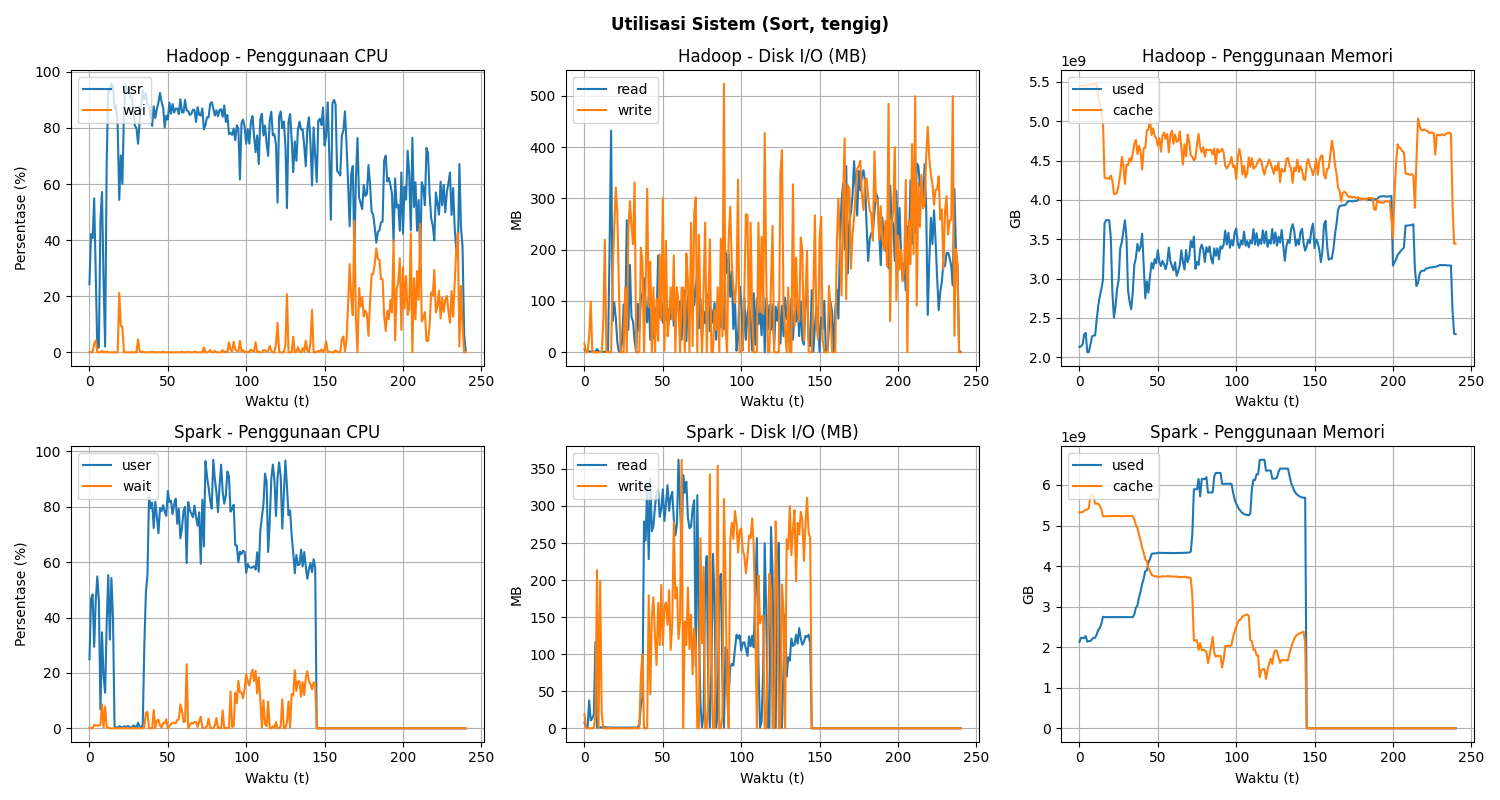
\includegraphics[width=0.9\textwidth]{figures/ch04/5-util-sistem-sort-tengig.png}
    \caption*{Sort, 10 GB}
\end{figure}

\begin{figure}[h]
    \centering
    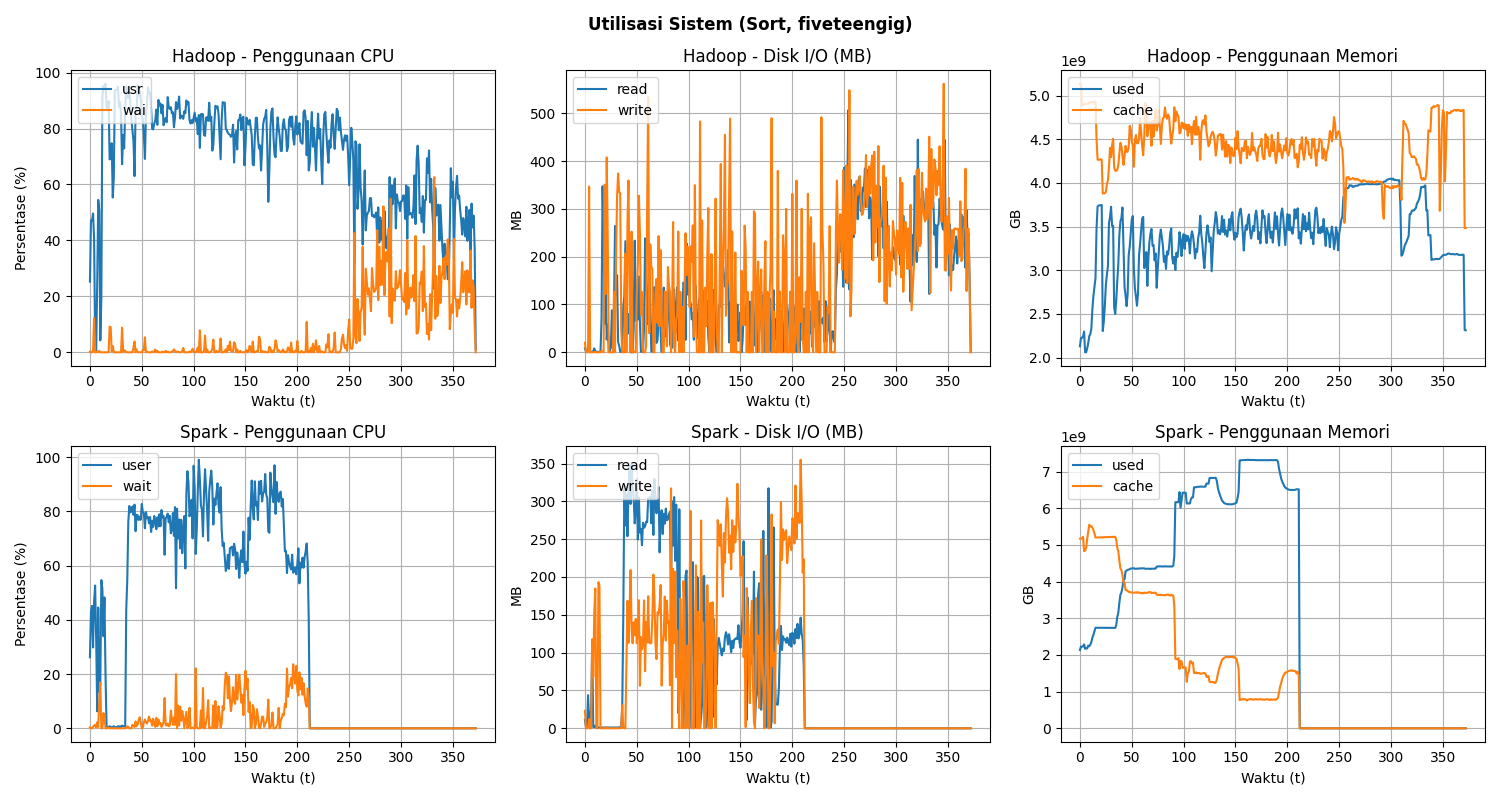
\includegraphics[width=0.9\textwidth]{figures/ch04/5-util-sistem-sort-fiveteengig.png}
    \caption*{Sort, 15 GB}
\end{figure}



%-------------------------------------------------


\chapter{Visualisasi Utilisasi Sistem Sesuai Input Data (\textit{Word Count})}
\label{appendix:H}

\begin{figure}[h]
    \centering
    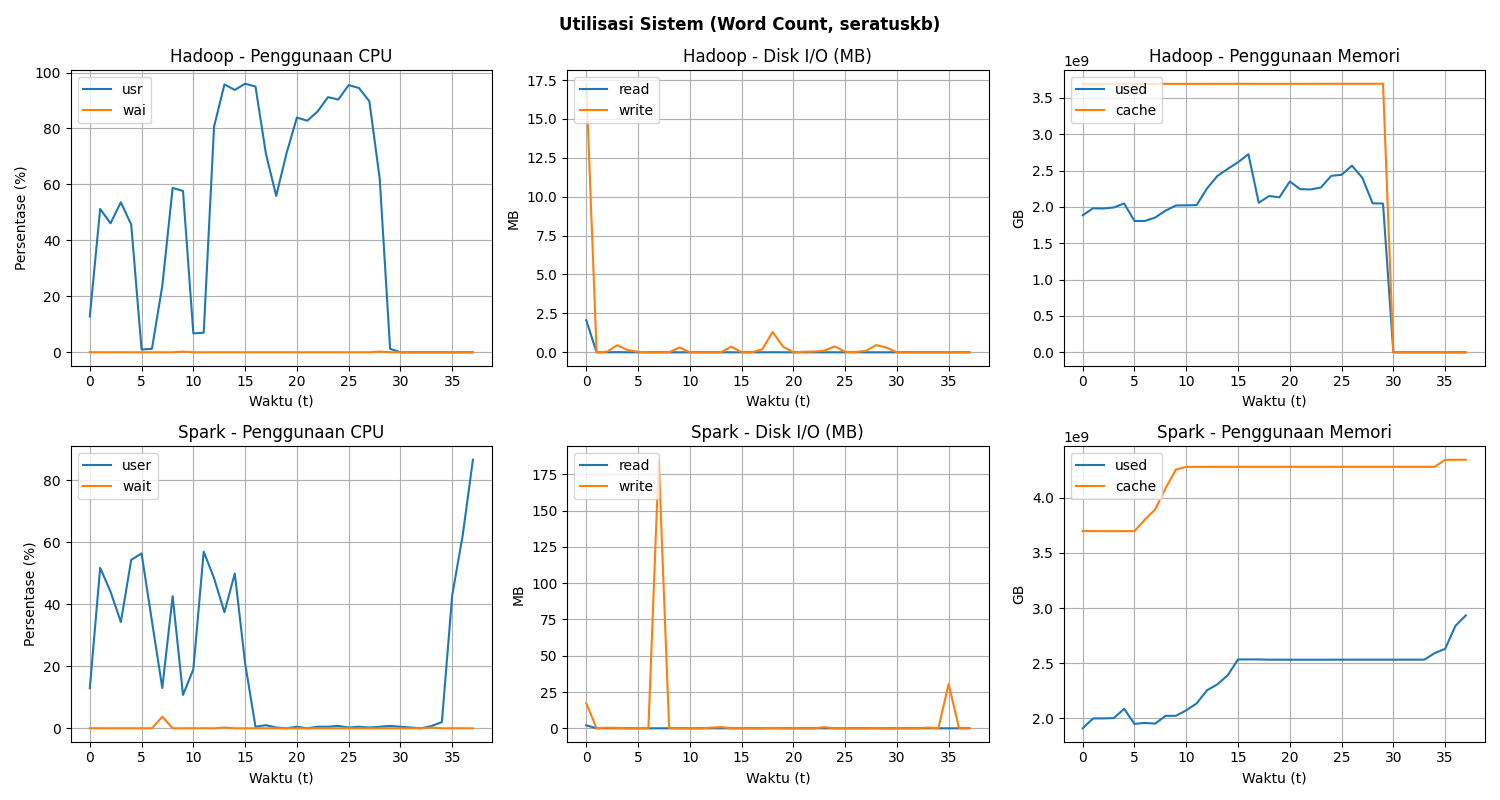
\includegraphics[width=0.9\textwidth]{figures/ch04/5-util-sistem-wordcount-seratuskb.png}
    \caption*{Word Count, 100 KB}
\end{figure}

\begin{figure}[h]
    \centering
    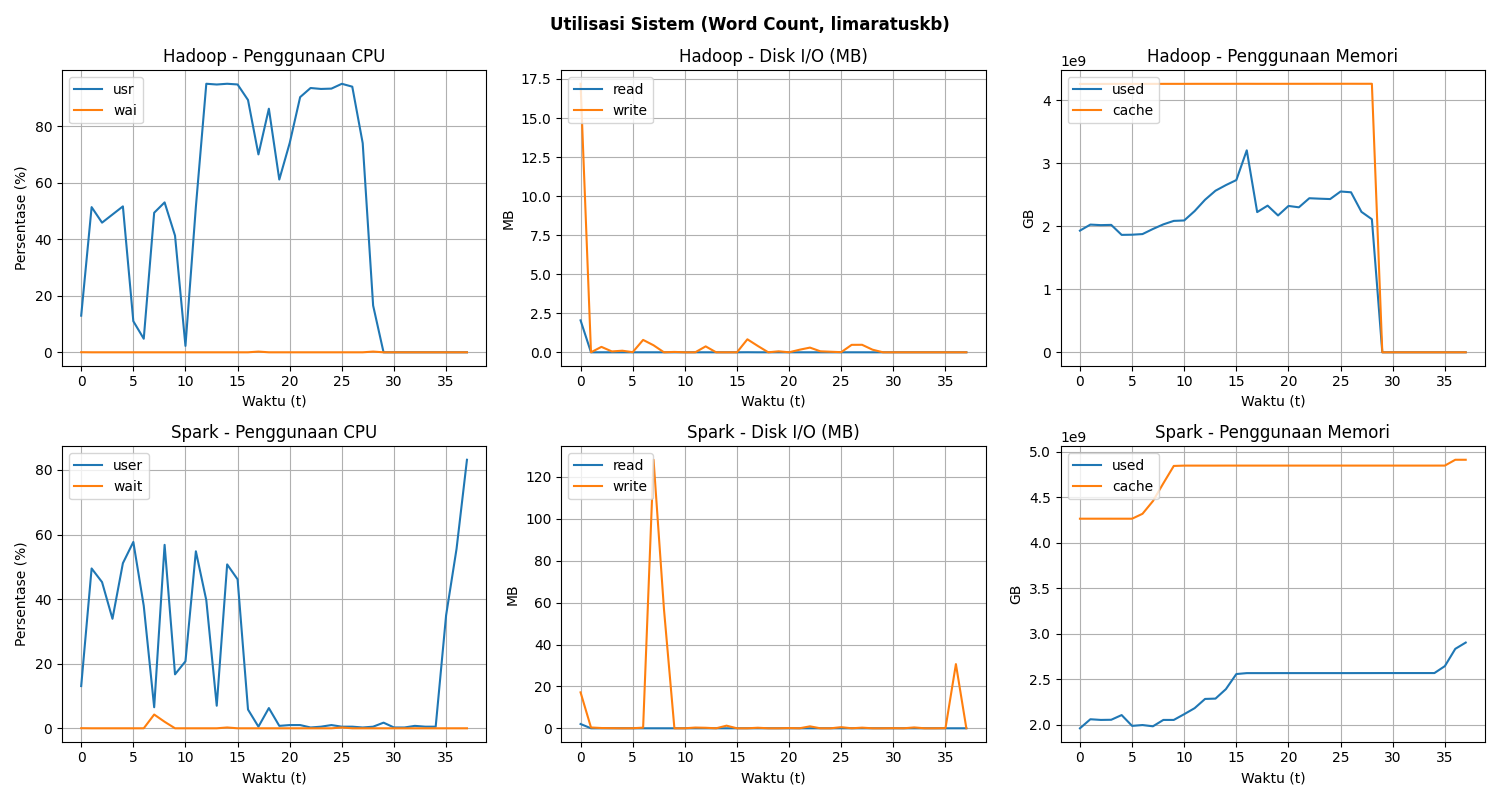
\includegraphics[width=0.9\textwidth]{figures/ch04/5-util-sistem-wordcount-limaratuskb.png}
    \caption*{Word Count, 500 KB}
\end{figure}

\begin{figure}[h]
    \centering
    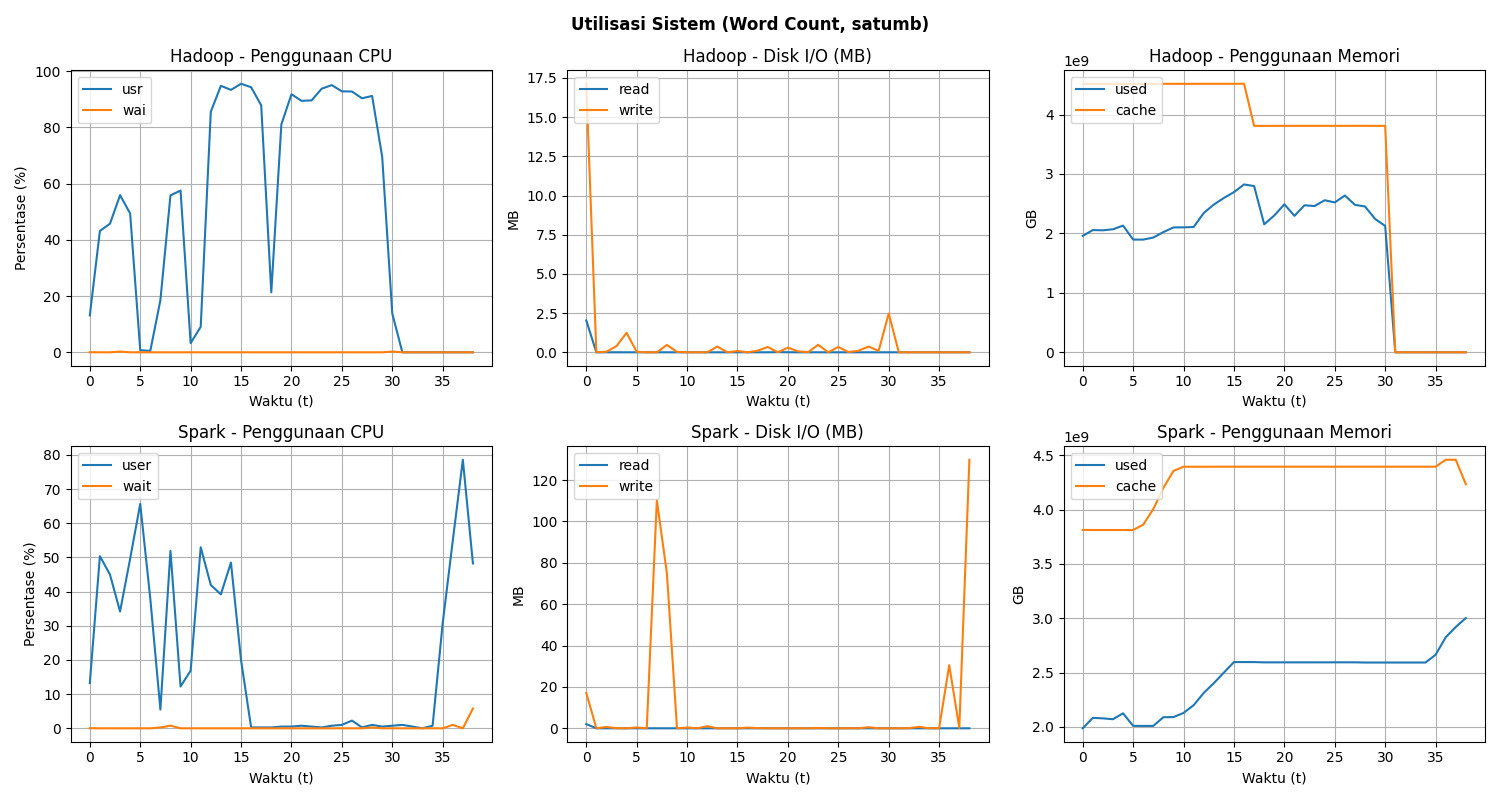
\includegraphics[width=0.9\textwidth]{figures/ch04/5-util-sistem-wordcount-satumb.png}
    \caption*{Word Count, 1 MB}
\end{figure}

\begin{figure}[h]
    \centering
    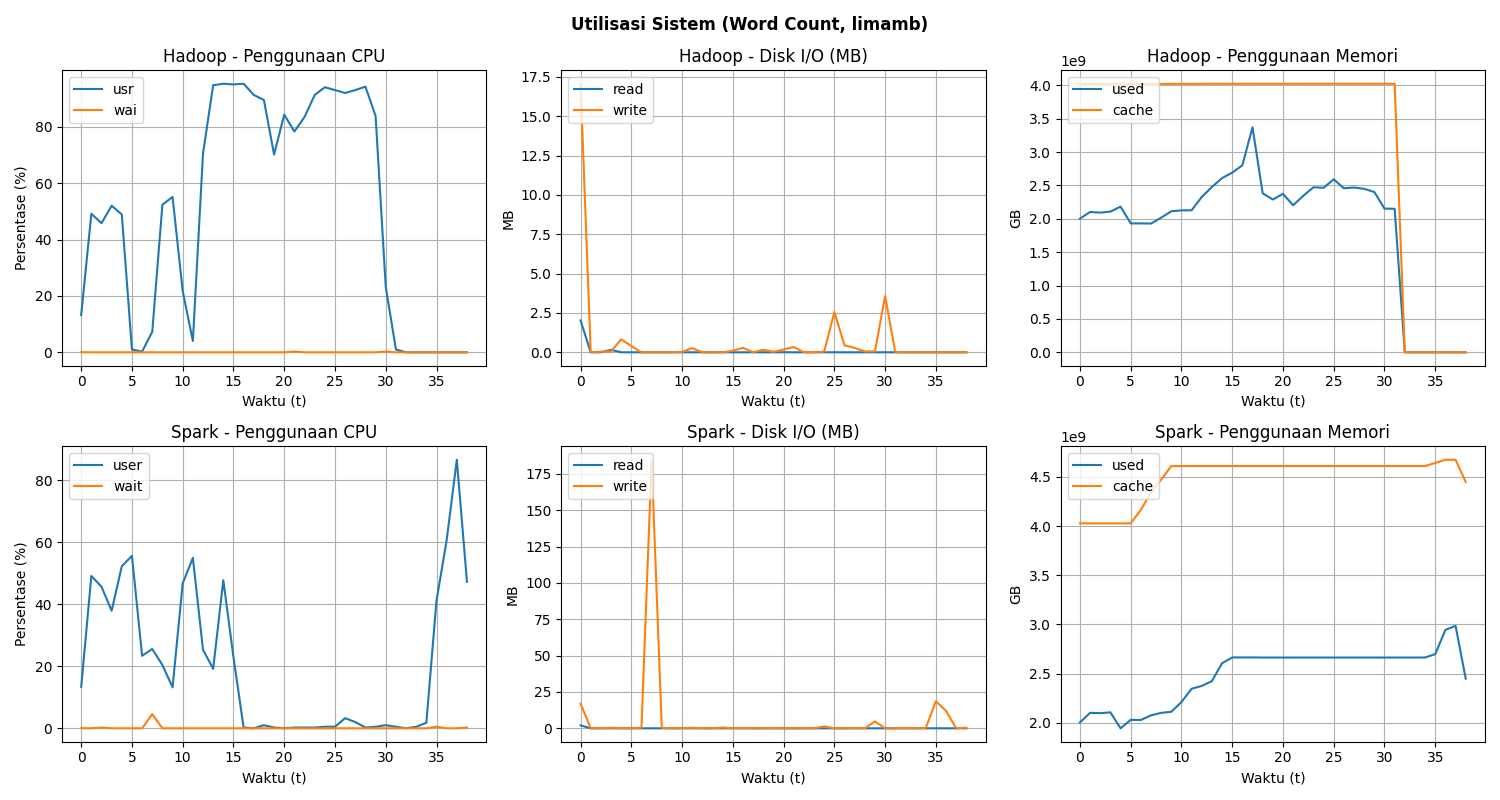
\includegraphics[width=0.9\textwidth]{figures/ch04/5-util-sistem-wordcount-limamb.png}
    \caption*{Word Count, 5 MB}
\end{figure}

\begin{figure}[h]
    \centering
    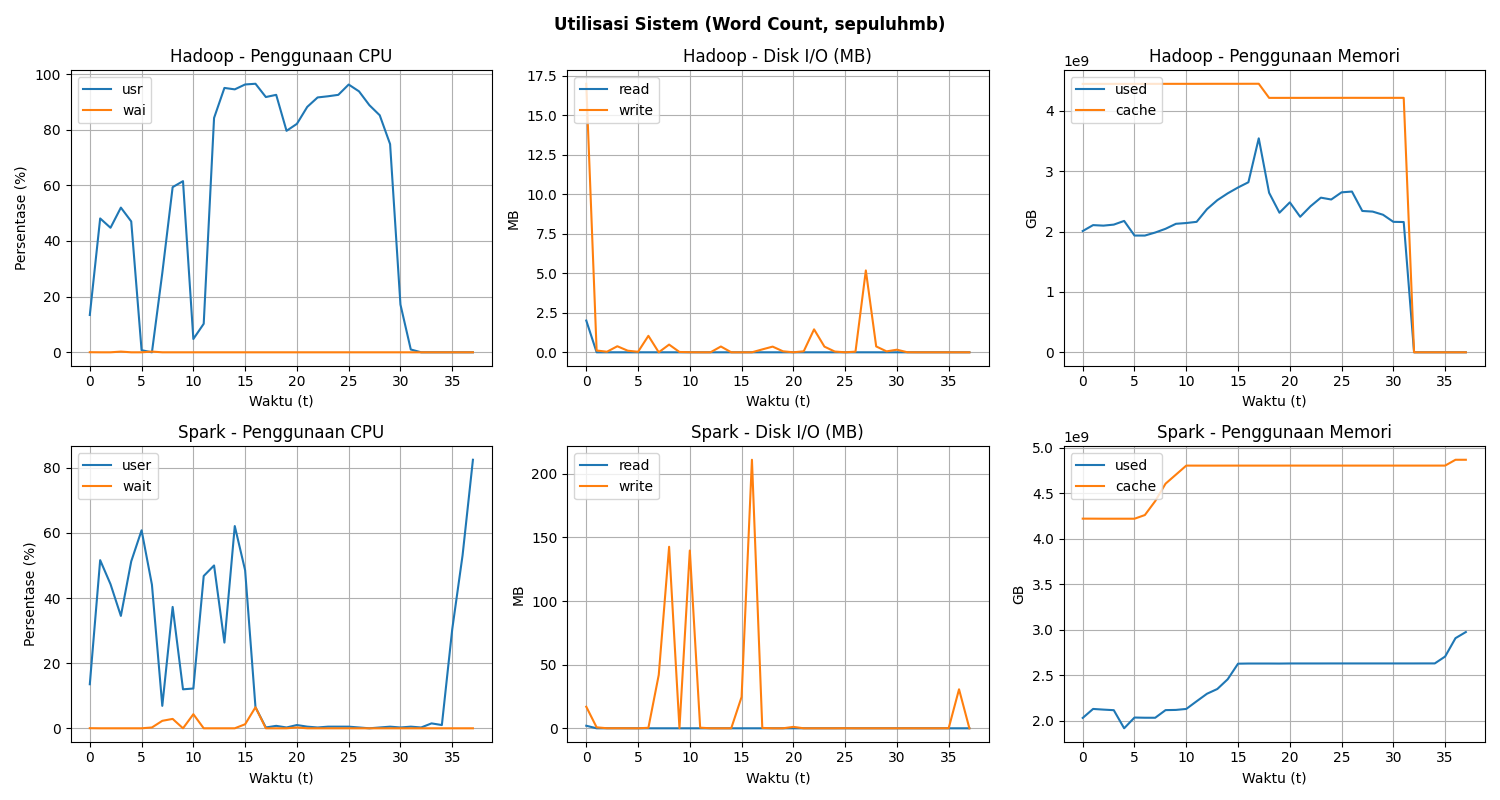
\includegraphics[width=0.9\textwidth]{figures/ch04/5-util-sistem-wordcount-sepuluhmb.png}
    \caption*{Word Count, 10 MB}
\end{figure}

\begin{figure}[h]
    \centering
    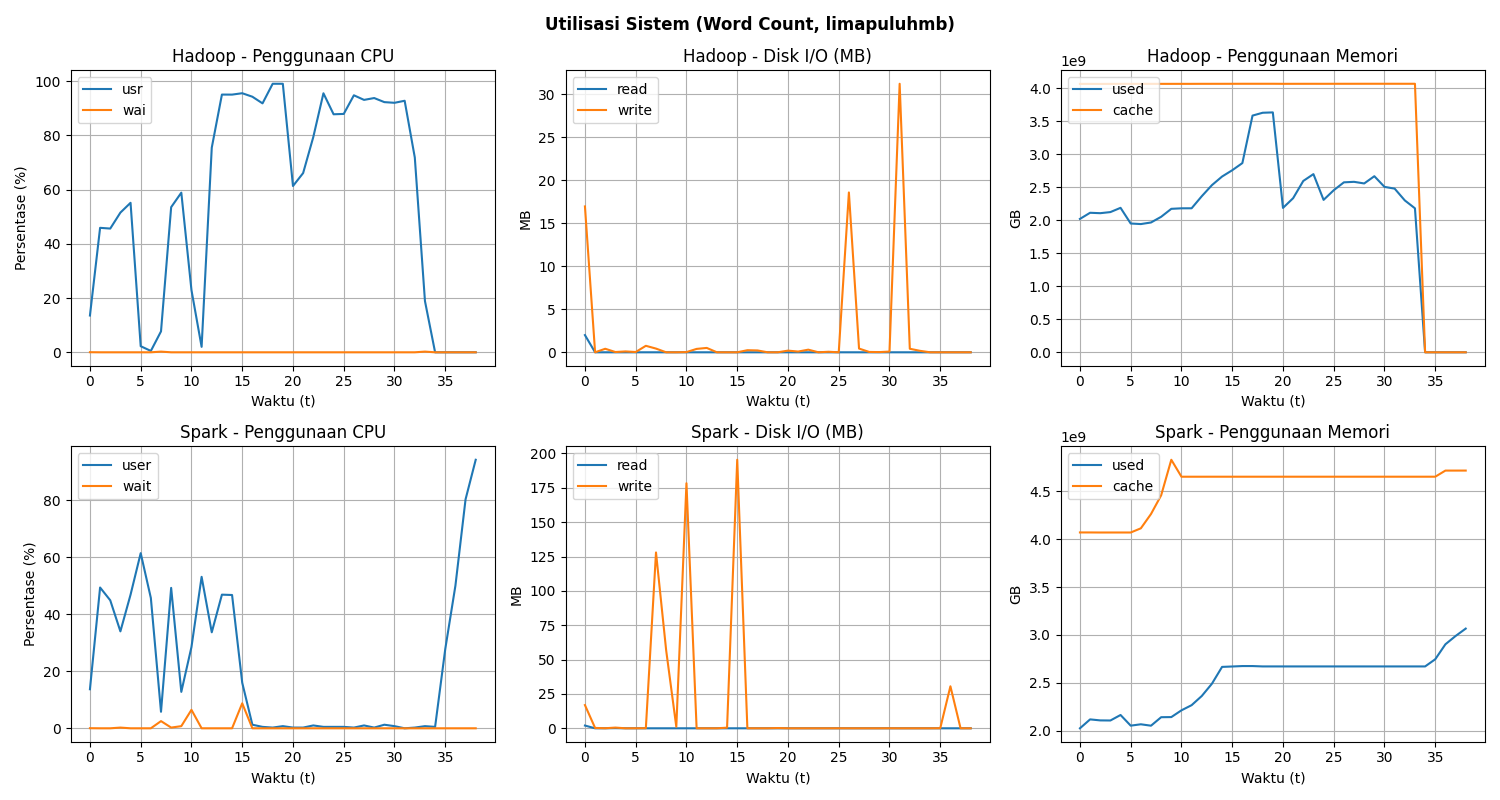
\includegraphics[width=0.9\textwidth]{figures/ch04/5-util-sistem-wordcount-limapuluhmb.png}
    \caption*{Word Count, 50 MB}
\end{figure}

\begin{figure}[h]
    \centering
    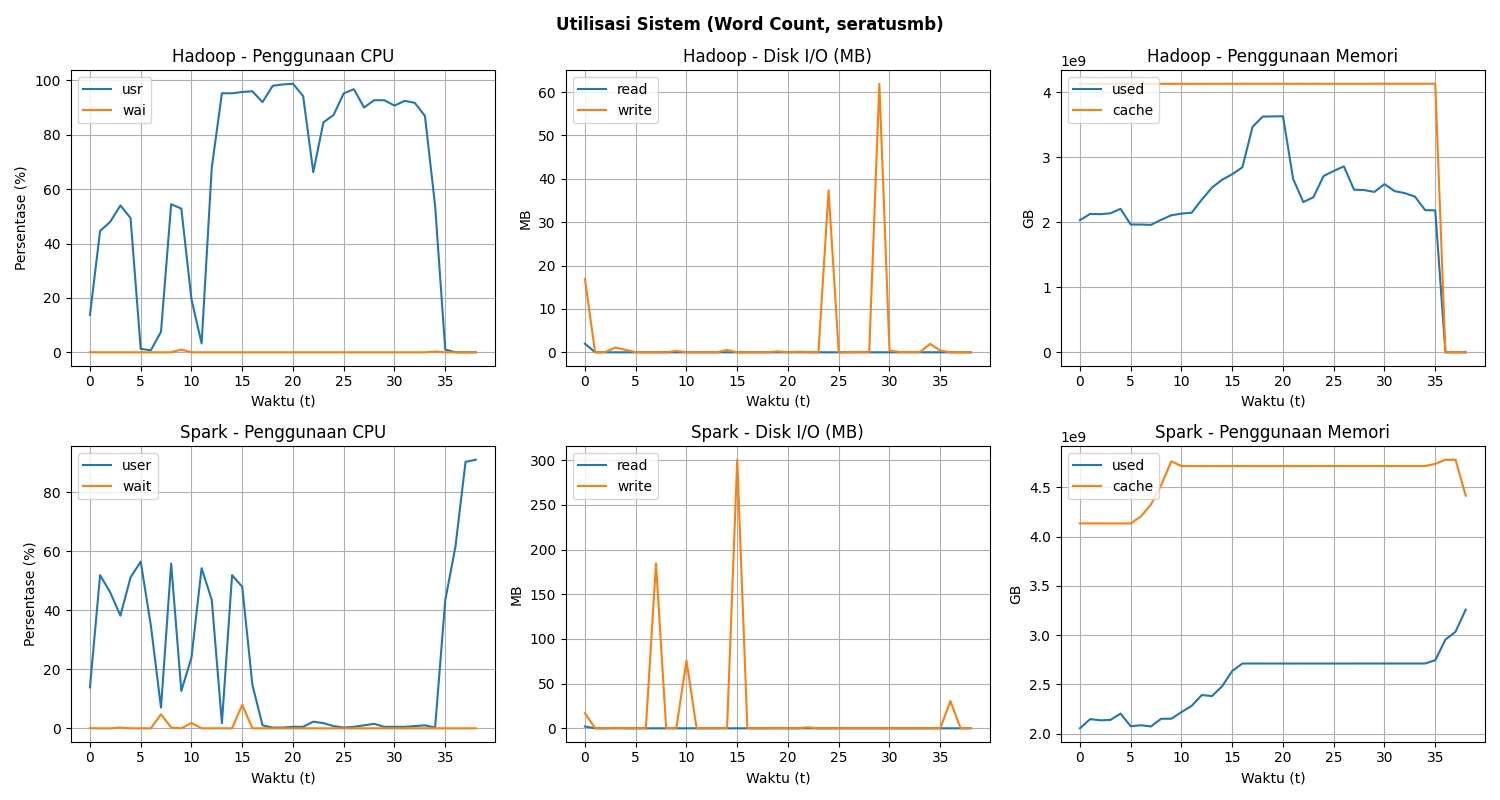
\includegraphics[width=0.9\textwidth]{figures/ch04/5-util-sistem-wordcount-seratusmb.png}
    \caption*{Word Count, 100 MB}
\end{figure}

\begin{figure}[h]
    \centering
    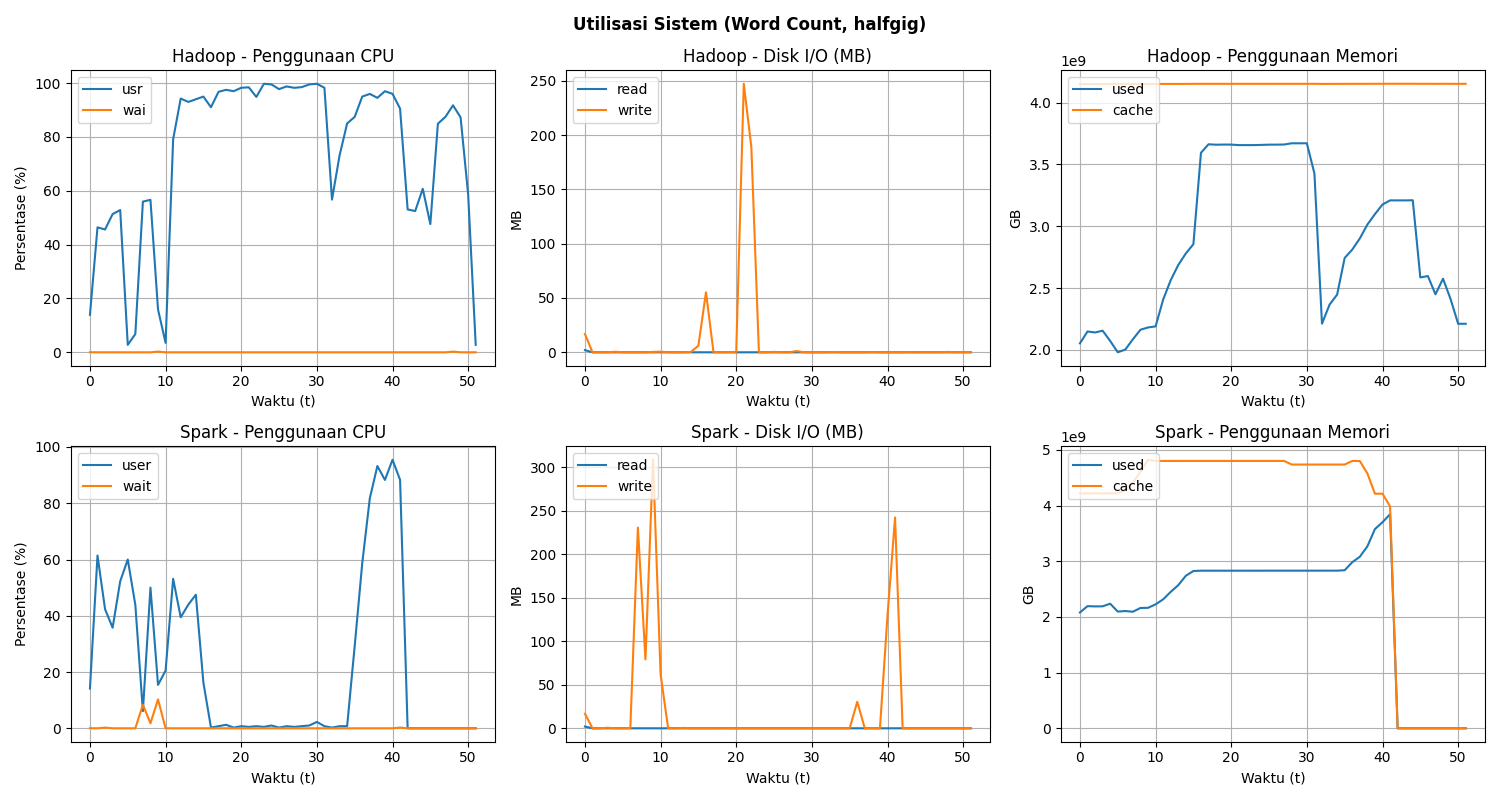
\includegraphics[width=0.9\textwidth]{figures/ch04/5-util-sistem-wordcount-halfgig.png}
    \caption*{Word Count, 500 MB}
\end{figure}

\begin{figure}[h]
    \centering
    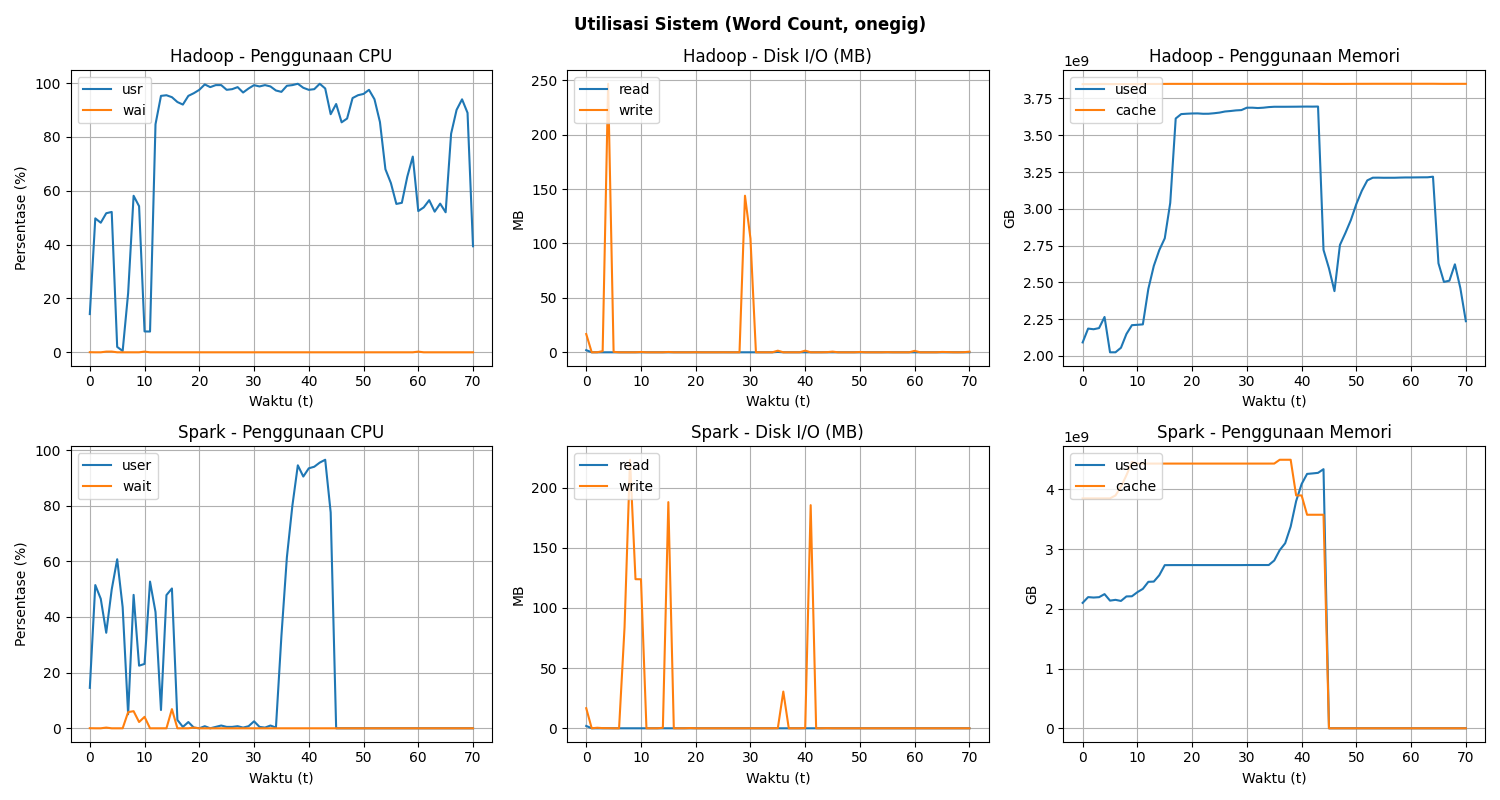
\includegraphics[width=0.9\textwidth]{figures/ch04/5-util-sistem-wordcount-onegig.png}
    \caption*{Word Count, 1 GB}
\end{figure}

\begin{figure}[h]
    \centering
    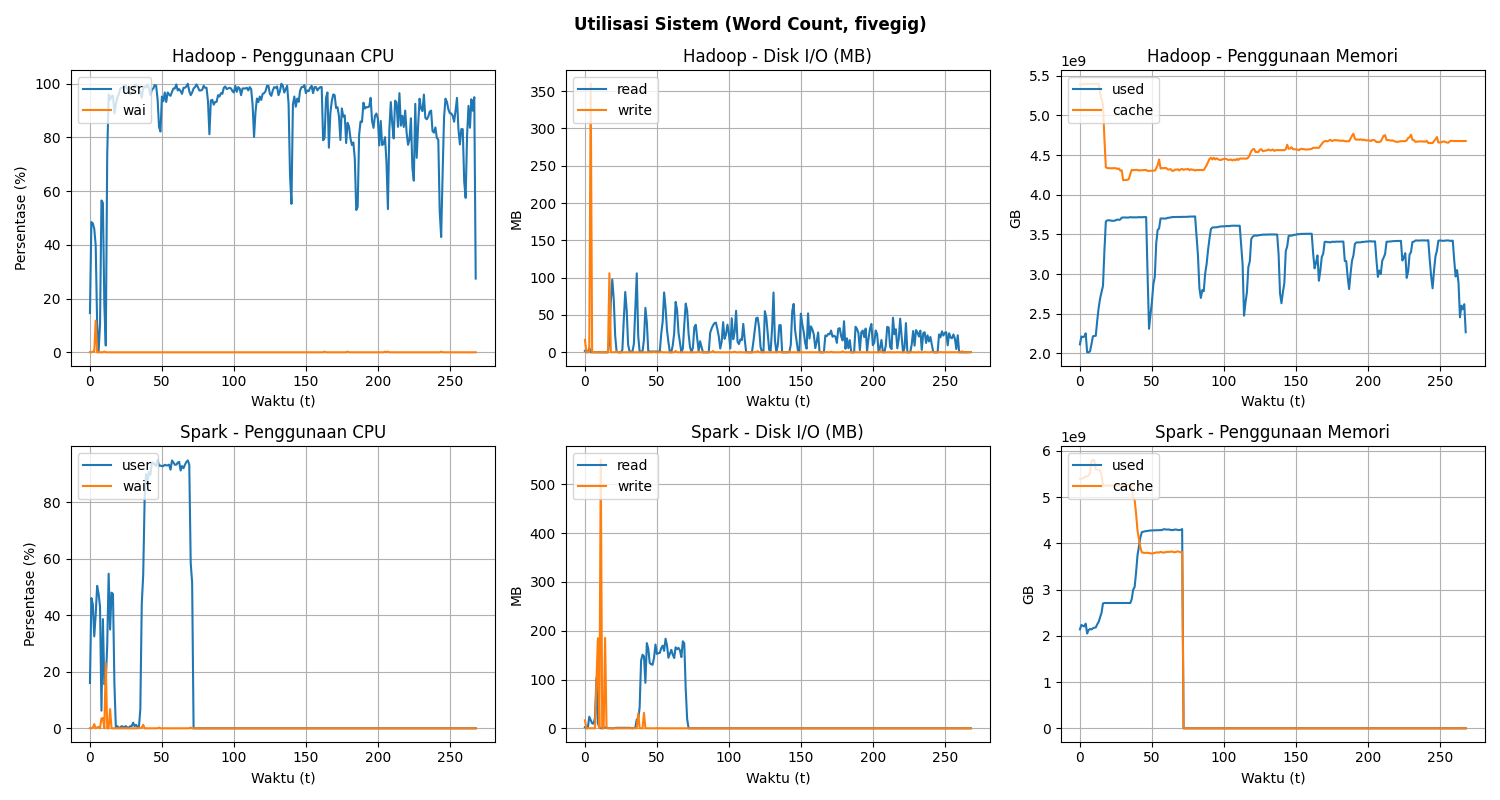
\includegraphics[width=0.9\textwidth]{figures/ch04/5-util-sistem-wordcount-fivegig.png}
    \caption*{Word Count, 5 GB}
\end{figure}

\begin{figure}[h]
    \centering
    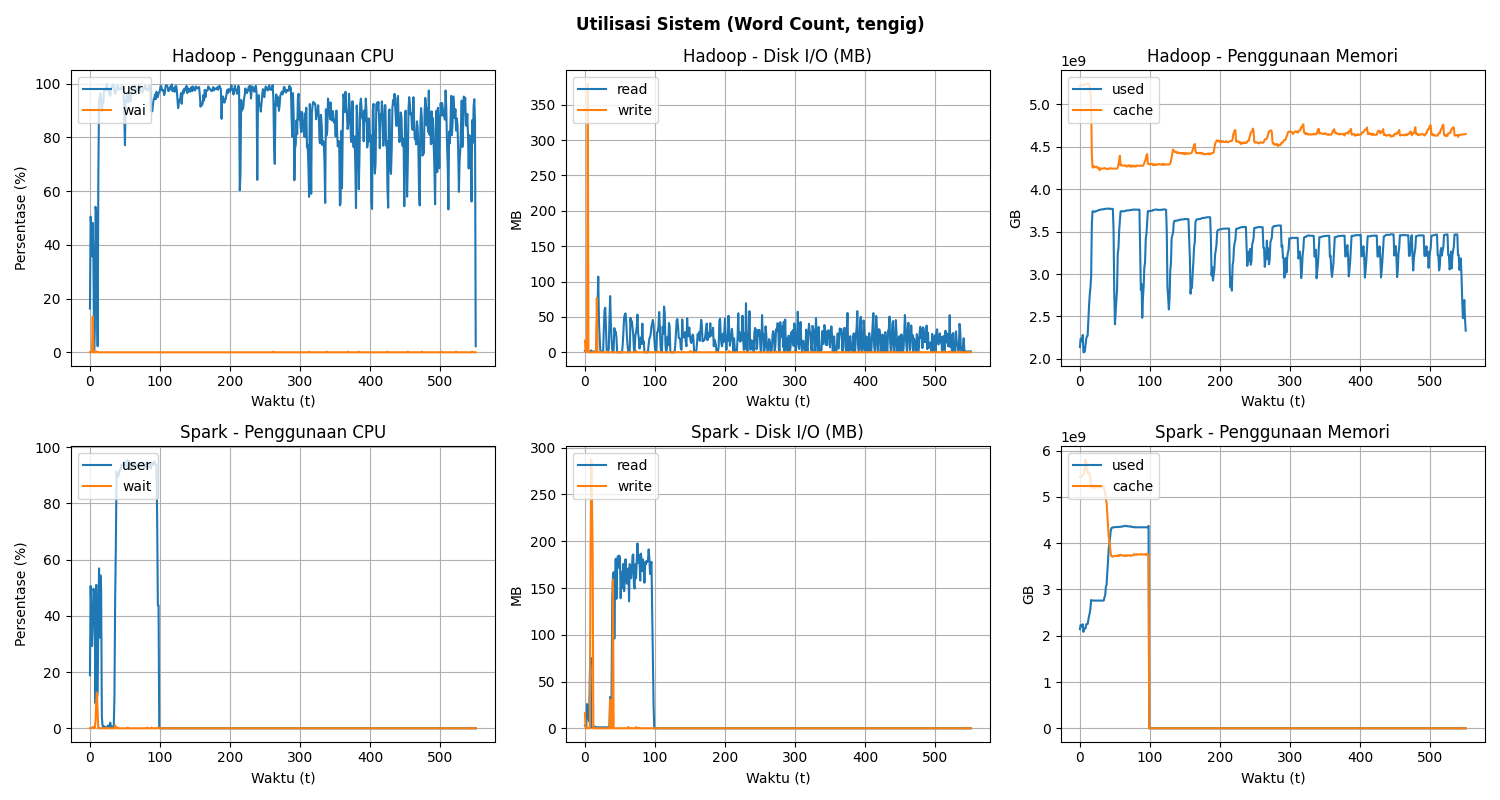
\includegraphics[width=0.9\textwidth]{figures/ch04/5-util-sistem-wordcount-tengig.png}
    \caption*{Word Count, 10 GB}
\end{figure}

\begin{figure}[h]
    \centering
    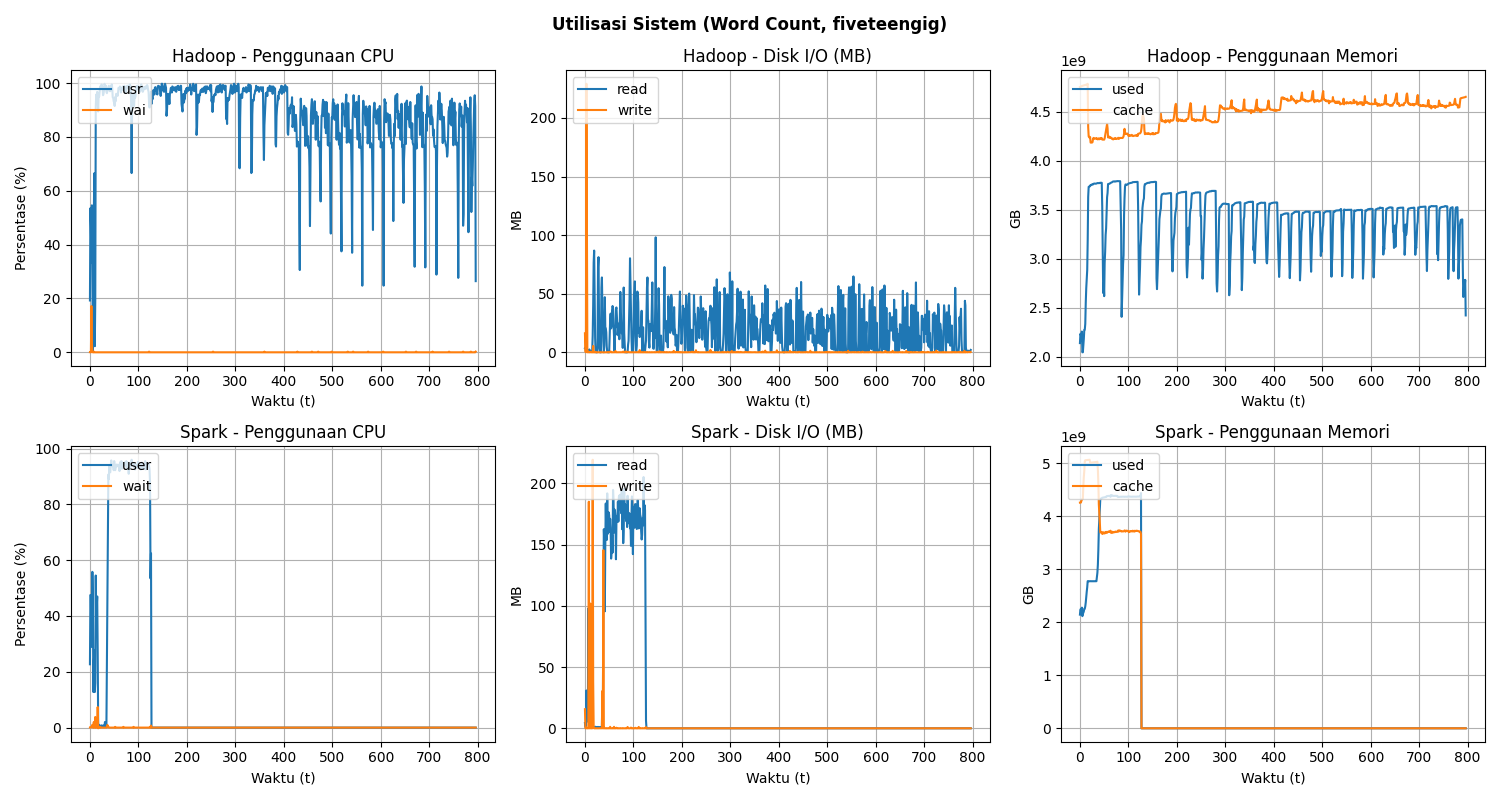
\includegraphics[width=0.9\textwidth]{figures/ch04/5-util-sistem-wordcount-fiveteengig.png}
    \caption*{Word Count, 15 GB}
\end{figure}
